\documentclass[a4paper, 12pt, oneside]{report}

\usepackage[utf8]{inputenc}
\usepackage{lmodern}
\usepackage{layout}
\usepackage{emptypage}
\usepackage{fancyhdr}
\usepackage{graphicx}
\usepackage{subfigure}
\usepackage{caption}
\usepackage{mathtools}
\usepackage{hyperref}
\usepackage[a4paper,top=3cm, bottom=3cm, inner=2.5cm, outer=2.5cm]{geometry}
\usepackage{listings}
\usepackage[british]{babel}
\usepackage{url}
\usepackage{float}
\usepackage{multirow}
\usepackage{rotating} 
\usepackage{color}
\usepackage{colortbl}
\usepackage{amsmath}
\usepackage{amssymb}
\usepackage[table]{xcolor}
\usepackage{algorithm}
\usepackage{algpseudocode}
\usepackage{comment}

\setlength{\parindent}{0pt}
\newcommand\abs[1]{\left|#1\right|}

\usepackage[utf8]{inputenc}

\usepackage{dirtytalk}
\usepackage{float}
\usepackage{verbatim}

\newcommand{\etal}{\textit{et al}. }

\makeatletter
\renewcommand{\@makeschapterhead}[1]{%
%  \vspace*{50\p@}%
  \vspace*{0\p@}%
  {\parindent \z@ \raggedright
    \normalfont
    \interlinepenalty\@M
    \Huge \bfseries  #1\par \nobreak
%    \vskip 40\p@
    \vskip 15\p@
  }}
\makeatother

\renewcommand{\baselinestretch}{1.4}
\setlength{\headheight}{16pt} 
\captionsetup{justification=justified}
\pretolerance=1000

\chead[]{}
\rhead[]{}
\renewcommand{\headrulewidth}{0.5pt}

\pagestyle{empty}

\title{Multiobject tracking using deep learning and tracking by detection}
\author{Alexandre Rodriguez Rendo}

\lstset{
	float=hbp,
	basicstyle=\ttfamily\small,
	columns=flexible,
	tabsize=4,
	frame=single,
	extendedchars=true,
	showspaces=false,
	showstringspaces=false,
	numbers=none,
	numberstyle=\tiny,
	breaklines=false,
	breakautoindent=true,
	captionpos=b
}
\setcounter{tocdepth}{4}
\setcounter{secnumdepth}{4}

\definecolor{lightgray}{gray}{0.9}

\begin{document}
%%%%%%%%%%%%%%% Portada %%%%%%%%%%%%%%%%%%%%
\begin{titlepage}
	
	\begin{center}
		\vspace*{7.7mm}
		\begin{center}
			
\includegraphics[width=0.4\linewidth]{figures/logo.jpg}
		\end{center}
		\vspace{6.5mm}
		
		\fontsize{15.5}{14}\selectfont ESCUELA TÉCNICA SUPERIOR DE INGENIERÍA DE TELECOMUNICACIÓN
		\vspace{13mm}
		
		\fontsize{14}{14}\selectfont MASTER OFICIAL EN VISIÓN ARTIFICIAL 
		
		\vspace{70pt}
		
		\fontfamily{lmss}\fontsize{15.7}{14}\selectfont \textbf{Master thesis} 
		
		\vspace{25mm}
		\begin{huge}
			Multiobject tracking using deep learning and tracking by detection
		\end{huge}
		
		\vspace{25mm}
		
		\begin{large}
			Author: Alexandre Rodríguez Rendo
			
			Tutor: José María Cañas Plaza
						
			\vspace{10mm}
		\end{large}
		\begin{normalsize}
			Academic course 2018/2019		
		\end{normalsize}
		\vspace{10mm}
		
	\end{center}
	
\end{titlepage}

\pagebreak
\thispagestyle{empty}
\vspace*{12cm}

\begin{comment}
\begin{flushright}

\includegraphics[height=1.0cm]{figures/CC-BY-SA.png}

\vspace*{0.5cm}

\copyright 2017 Marcos Pieras Sagardoy

\vspace*{0.3cm}

Esta obra está distribuida bajo la licencia de 

``Reconocimiento-CompartirIgual 4.0 Internacional (CC BY-SA 4.0)''

de Creative Commons.

\vspace{0.2cm}

Para ver una copia de esta licencia, visite

http://creativecommons.org/licenses/by-sa/4.0/ o envíe

una carta a Creative Commons, 171 Second Street, Suite 300,

San Francisco, California 94105, USA.

\end{flushright}
\end{comment}

\pagenumbering{Roman}

%%%%%%%%%%%%%%% Agradecimientos %%%%%%%%%%%%
\chapter*{Acknowledgement}
\textit{Galician version}\\
En primeiro lugar quero dar as grazas ao meu titor Jose María polo apoio e axuda neste proxecto. Por outra banda, agradecer a amig@s, compañeir@s de estudo, de traballo, de vivenda... tod@s os que me acompañaron e animaron neste camiño.\\
Aos meus avós, os que están e os que xa non están pero seguen preto, por ser o maior exemplo de humanidade que un pode ser. Sen vós non sería nada do que son agora. Gracias de verdade.\\
A Cintia por ser á vez psicóloga, amiga e irmá.\\
Especialmente aos meus pais que me ensinaron a importancia de palabras como traballo, honestidade e valores. A partir do que vós me ensinastes fun capaz de poder aprender moitas cousas mais. Quérovos moito!\\
Seguramente me falte moita xente por mencionar pero creo que aquí está o máis importante.\\ \ \\
\textit{English version}\\
First of all I would like to thank my tutor Jose Maria for the support and help in this project. On the other hand, I would like to thank friends, colleagues, work colleagues, flat mates ... everyone who accompanied me and encouraged me on this path. \\
To my grandparents, those who are and those who are no longer but there are still close, for being the greatest example of humanity that one can be. Without you there I would not be what I am now. Thank you really. \\
To Cintia for being a psychologist, friend and sister at the same time. \\
Especially to my parents who taught me the importance of words such as work, honesty and values. From what you taught me I was able to learn many more things. I love you! \\
Surely I miss many people to mention but I think that here are the most important ones.


%%%%%%%%%%%%%%% Resumen %%%%%%%%%%%%%%%%%%%%
\chapter*{Abstract}
The visual multiple object tracking is an open problem inside the computer vision community with multiple applications in the industry such as in the autonomous vehicles or in the security field. Many efforts has been made in the past to solve this task, especially for person tracking due to its greater interest.\\
In the last years, the deep learning techniques have been able to beat the state of the art in tasks such as image classification or object detection in images. Thus, this work has made use of deep learning methods to built a visual multiobject tracking application. These techniques are combined with a tracking by detection scheme to perform the tracking and achieve a good balance between speed and accuracy in the tracking. The final developed software component, named as \textit{dl-objecttracker}, has a mechanism of tracking processing speed measurement that allows for different tracking processing speed regimes and it is also configurable.\\
Finally, the developed solution has been experimentally validated on the MOT17Det dataset, one of the most well-known datasets of multiple object tracking (MOT).



%%%%%%%%%%%%%%% Índices %%%%%%%%%%%%%%%%%%%%
\renewcommand{\tablename}{Table}
\renewcommand{\listtablename}{List of Tables}
\tableofcontents

\cleardoublepage % Índice de figuras
\addcontentsline{toc}{chapter}{\listfigurename}
\listoffigures

\cleardoublepage % Índice de tablas
\addcontentsline{toc}{chapter}{List of Tables}
\listoftables 

\cleardoublepage
%%%%%%%%%%%%%%% Capítulos %%%%%%%%%%%%%%%%%%
\pagestyle{fancy}
\pagenumbering{arabic}
\setlength{\parindent}{6mm}

\lhead[]{CHAPTER \thechapter. Introduction}
\chapter{Introduction}\label{cap.introduccion}
\setlength{\parindent}{0pt}
The Multiple Object Tracking or \textit{MOT} is an important computer vision problem which continues to attract attention because of its potential in both the academic and commercial spheres. The real-world applications of the multiobject tracking are numerous including human-computer interaction, autonomous vehicles, robotics, video indexing, surveillance or security, among others. The computer vision community have been making efforts in the past few decades but the MOT task is still open for improvement. One of the most studied tracking areas is the pedestrian tracking, mainly because the videos of pedestrians can be seen in a large number of applications with commercial potential. As some studies indicate [1], about the 70\% of the current research done in MOT is dedicated to pedestrians. The difficulty of MOT lies in various challenging situations that can occur such as variation of the illumination and the scale, target deformation or fast motion. Most of this challenges are common to Single Object Tracking (\textit{SOT}) but MOT also needs to solve two main tasks: determining the number of objects that usually vary over time and mantaining their identities.
\section{Objectives}


\lhead[]{CHAPTER \thechapter. State of the Art}
\chapter{State of the Art}\label{cap.estadodelarte}
\setlength{\parindent}{0pt}
\section{Neural Networks in Computer Vision}
Since the birth of Artificial Intelligence (AI) in 1956, the computer vision has followed a great rhythm of evolution. Taking the machines to equal humans in the resolution of some tasks, and in certain cases, to overcome them.
Artificial intelligence is defined in ~\cite{mccarthy2006proposal} as ``the subfield of Computer Science dedicated to developing programs that allow computers to present behaviors that can be characterized as intelligent". Machine learning (\textit{ML}) is defined in ~\cite{samuel2000some} as ``a field of Computer Science that gives computers the ability to learn without being explicitly programmed". Therefore, given this definition, the ML can be considered a subfield of the AI.\\
One of the most well known and currently growing ML subfields is called \textit{Deep Learning} ~\cite{deng2014deep}. This type of algorithm is intimately linked with the Artificial Neural Networks (\textit{ANN}) and in practice they are usually used in an equivalent way although they are not the same. One of the aspects to be highlighted in the Deep Learning algorithms is that it is no longer necessary to extract feature vectors for the input to the network. This is because these algorithms ``learn" how to represent the data in a hierarchical way. From these networks, the convolutional neural networks have a special interest to face the problem that this project presents. This type of networks are characterized by the use of a convolution operation in at least one of the layers of the network and their design for the processing of two-dimensional data such as images ~\cite{liu2015implementation}. In recent years, its evolution has been constant being able to overcome the results achieved by previous algorithms in tasks such as object classification and detection.\\

\subsection{Object classification and detection using neural networks}
Much of the progress made in recent years on the classification field of computer vision can be directly associated with a set of neural network architectures. The first big step forward came in 2012 when AlexNet ~\cite{krizhevsky2012imagenet} beats all the proposals of the state of the art at that time in the ImageNet challenge, ILSVRC. This competition of classification in images is a reference in the computer vision community. AlexNet obtained a test error rate of 15.3\% compared to the previous year's winner which was 26.2\%. This network, together with the VGG networks ~\cite{simonyan2014very}, follows the basic design archetype of convolutional networks: a series of convolution layers, followed by max-pooling and activation layers before the final classification layers \textit{fully-connected}. MobileNet is a simplified version of Xception ~\cite{chollet2016xception} for mobile applications that is currently behind the computer vision applications used on Google mobile devices.\\
The ResNet and Inception architectures, among others, are been used as blocks that serve as the basis for numerous subsequent works in computer vision and are briefly commented below:
\begin{itemize}
\item \textbf{Res-Net} ~\cite{he2016deep}: this network tries to solve the problem that seems to appear when adding layers to a network and that is that it generally behaves worse. For this reason, the authors propose that instead of trying to learn the hidden \textit{mapping} of the input \textit{x} to the function \textit{H(x)}, learn the difference between the two, that is, the residue (\textit{residual net}). For the calculation of H(x) they simply add the residue to the input and re-enter the next layer. This is a big change at the time as it solves the problem of the \textit{vanishing gradients} that the neural networks have suffered until the date. In addition, it allows to create much deeper networks, that is to say, with more layers, that allow better results.
\item \textbf{Inception} ~\cite{szegedy2015going}: this family of networks looks for wider networks, that is, with more intermediate operations between layers. The authors try to increase neural networks, in terms of operations, without an increase in computational cost. Introducing different parallel convolution operations the density of extracted information increases but also the computational costs. To solve the problem they use 1x1 convolutions to reduce dimensionality while performing different transformations in parallel. The resulting networks are simultaneously deep and wide.\\
The first version of Inception, known as GoogLeNet, was the winner of the 2014 ILSVRC. It was improved later with Inception v2 and v3. The last Inception v4 creates a hybrid with ResNet, known as Inception-ResNet ~\cite{szegedy2017inception}.
\end{itemize}
With the arrival of autonomous vehicles, intelligent video surveillance, face detection and numerous emerging applications, faster and more accurate detection systems are increasingly in demand. This includes not only recognizing and classifying each object in the image but also locating it with its corresponding text{bounding box}. This makes object detection significantly more complicated than traditional image classification. However, the most successful object detection algorithms today are extensions of image classification models.\\
The main object detection models are then introduced ~\cite{fu2017dssd}.  %cambiar: modify classification to remark difference between regionbased and singleshot
\begin{itemize}
    \item \textbf{Faster R-CNN} ~\cite{ren2015faster}: is one of the current reference models and one of the last detectors known as  \textit{region-based} from Girshick \etal{}This models basically work in the following way: they use some mechanism to extract regions from an image that are probably an object and then classify those proposed regions with a CNN. The father of this model is the R-CNN and it was the real driver of this type of techniques ~\cite{girshick2014rich}. In the proposed regions obtained through an algorithm called \textit{Selective Search} the characteristics are extracted through a CNN by region and then those regions are classified based on the characteristics. But its performance was slow.\\
    This performance improves with Fast R-CNN ~\cite{girshick2015fast} for two main reasons. The first is that the CNN is applied over the whole image instead of over each region and then the regions are obtained from the last map of characteristics of the network. The second is due to the introduction of a Softmax layer that simplifies classification. Its mechanism was faster and easier to train than R-CNN but there was still a bottleneck in the generation of regions.\\
    To solve it the RPN (\textit{Region Proposal Network}) is introduced and added to the Fast R-CNN it creates Faster R-CNN. The RPN returns proposed regions based on a \textit{score} that refers to the probability that the bounding box is an object, the \textit{objectness} (Figure \ref{fig:fasterrcnn}). And these regions are passed directly to the Fast R-CNN.\\
    \begin{figure}[h!]
    \begin{center}
    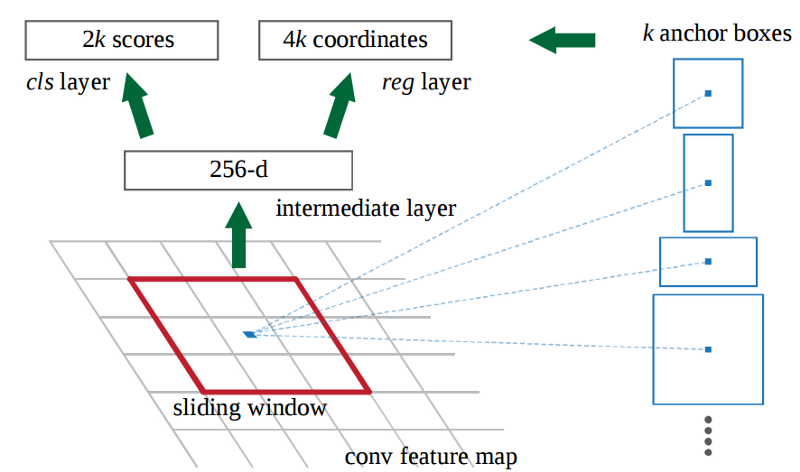
\includegraphics[scale=0.25]{faster_rcnn.png}
    \caption{Region Proposal Network (RPN)}
    \label{fig:fasterrcnn}
    \end{center}
    \end{figure}
\item \textbf{Overfeat} ~\cite{sermanet2013overfeat}: winner of the ILSVRC 2013 in location and detection of objects, this work showed that training a convolutional network to simultaneously classify, locate and detect objects in images can enhance the success both in classification, detection and location. Subsequently, it has been replaced by SSD and YOLO for tasks that require better detection in real time.
\item \textbf{R-FCN} ~\cite{dai2016r}: there are faster models than Faster R-CNN such as R-FCN, which tries to improve system speed by maximizing shared computing.
\item \textbf{SSD} ~\cite{liu2016ssd}: it provides great speed gains over Faster R-CNN by performing the phases of generating regions of interest and subsequent classification jointly (\textit{Single Shot MultiBox Detector}). As a result you get a lot of bounding boxes which most of them are not useful. By applying the techniques \textit{non-maximum suppression} and \textit{hard-negative mining} the final detections are achieved.
\item \textbf{YOLO} ~\cite{redmon2016yolo9000}: this model uses a different approach with respect to the above because it applies a single neural network to the entire image. This network divides the image into regions and predicts the bounding box and probabilities of each region. These are then weighted with the probabilities to obtain the definitive detections. This performs, as the authors indicate, a hundred times faster than Fast R-CNN maintaining a similar accuracy.\\
\end{itemize}
In the following table obtained from ~\cite{redmon2016yolo9000} it can be seen how YOLO is almost on a par with methods like SSD or Faster R-CNN. On the other hand, it has a better balance between speed and accuracy since it manages to work in some cases at 91 FPS (\textit{frames per second}) when Faster R-CNN barely reaches 10 FPS (see Table 3 in ~\cite{redmon2016yolo9000}).
\begin{table}[H]
\begin{center}
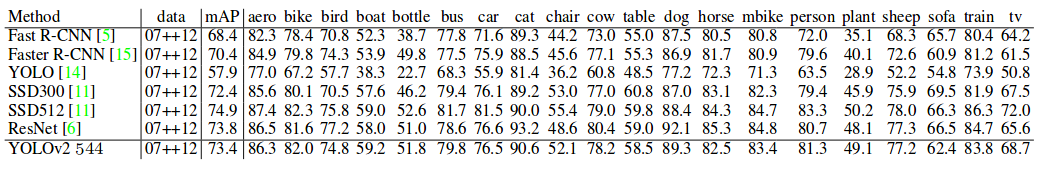
\includegraphics[scale=0.5]{yolo_results_pascal12.png}
\caption{Accuracy comparison in test phase in detection on PASCAL VOC 2012}
\end{center}
\end{table}
 The latest version of YOLO, called YOLOv3, achieves a 57,9 mAP on COCO test-dev. The frame rate is lower than the obtained with YOLOv2 (with the same image input size) but it still performs as a state-of-art real-time object detection system, according to the author \cite{redmon2018yolov3}.
\subsection{Segmentation using neural networks}
La comunidad en visión artificial ha mejorado los resultados obtenidos en detección de objetos y segmentación semántica en un corto período de tiempo gracias, en gran parte, a poderosos sistemas de base como Faster R-CNN. En este proyecto se tratará de realizar segmentación de instancias, lo cual requiere de la correcta detección de todos los objetos en la imagen junto con la segmentación precisa de cada instancia. Así, cada píxel pertenece a alguna de las diferentes categorías sin diferenciar que se encuentre o no en un determinado objeto.\\ %reescribir
Driven by the effectiveness of the R-CNN family many of the methods proposed for instance segmentation are based on segment proposals where segmentation precedes object type recognition ~\cite{pinheiro2015learning}. This has proved to be slower and more inaccurate than if the prediction of object masks and class labels were done in parallel and separately. Li \etal{} propose a system known as FCIS (\textit{Fully Convolutional Instance Segmentation}) ~\cite{li2016fully} that tries to predict the output of a set of position-sensitive channels in a completely convolutional way. These channels perform the tasks of class, bounding box and masks calculations simultaneously which makes them faster. But it shows errors in instances that overlap creating spurious edges systematically (Figure \ref{fig:fcis_mask}).
Recently, Mask R-CNN ~\cite{he2017mask} arose to solve many of these problems and to situate itself as a state-of-the-art technique in segmentation of instances as can be seen in Figure \ref{fig:fcis_mask}. Por ello esta sección se va a centrar en esta técnica y sus resultados.\\ %revisar se hai algo novo neste tema e definir segmentacion semantica, de instancias etc
\begin{figure}[H]
\begin{center}
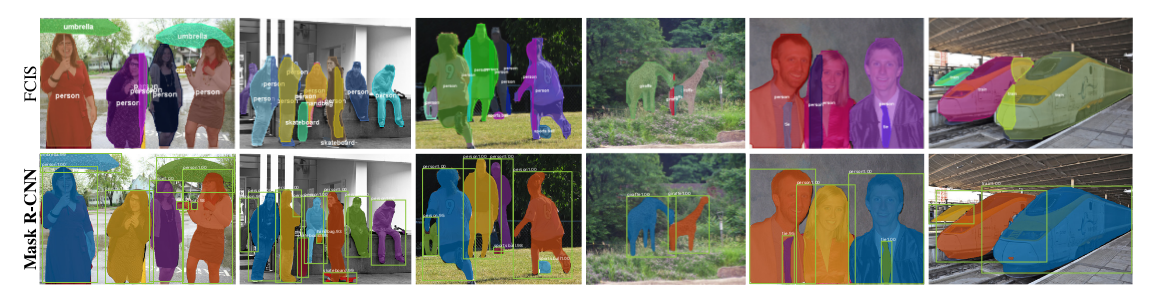
\includegraphics[scale=0.30]{fcis_vs_maskrcnn.png}
\caption{Results obtained by FCIS and Mask R-CNN in test images from COCO Dataset}
\label{fig:fcis_mask}
\end{center}
\end{figure}
Conceptually, Mask R-CNN adds a third stage to Faster R-CNN in which it obtains the mask of the object. The first stage of RPN coincides with that of Faster R-CNN while in the second stage it calculates, in parallel with the prediction of the class and the bounding box, a binary mask for each region of interest (\textit{RoI}). The generation of masks for each class is done without the classes competing with each other, which allows to separate the mask and class predictions from the object prediction. According to the authors, this proves to be the key to obtain good results in the final segmentation.\\ 
Another key factor in the proper functioning of this method is the correct alignment between the RoI and the extracted characteristics. This is usually done using \textit{RoIPool} in Fast R-CNN but introduces misalignments if the purpose is to segment rather than classify. This is why Mask R-CNN authors create \textit{RoIAlign}. To demonstrate the generality of the proposed method the authors introduce the mask prediction branch on several existing neural network architectures such as Faster R-CNN with ResNet as feature extractor, for example, and manage to surpass the winners of the 2015 and 2016 COCO Challenge segmentation, MNC ~\cite{dai2016instance} and FCIS ~\cite{li2016fully}. These experiments use COCO's standard metrics.\\
\begin{table}[h!]
\begin{center}
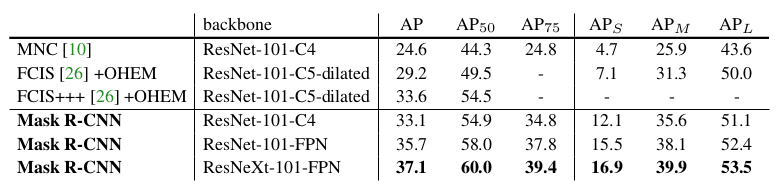
\includegraphics[scale=0.40]{mask_vs_mnc_fcis.png}
\caption{Results obtained from Mask R-CNN vs the previous works in segmentation on test images from COCO dataset}
\end{center}
\end{table}
As can be seen, all implementations of the Mask R-CNN model surpass the previous base models of the state of the art in instance segmentation.\\
Los autores también han realizado experimentos del rendimiento de esta técnica en el dataset Cityscapes (comentado en la sección 1.3). Para las categorías \textit{persona} y \textit{coche} este dataset presenta un gran número de instancias de diferentes clases solapadas, esto hace aún más complicada la correcta segmentación de instancias. Sin embargo, Mask R-CNN mejora los mejores métodos actuales en esta tarea y se convierte en método estado del arte. %necesario?
%------------------------------------------------------------------------
\subsection{Deep learning frameworks}
For the use of Deep Learning numerous \textit{frameworks} have emerged. A deep learning framework allows us to build deep learning models more easily and quickly, without getting into all the details of the underlying algorithms. Here are the frameworks used in this project:
\begin{itemize}
\item \textbf{Tensorflow}\footnote {\href{https://www.tensorflow.org/}{Tensorflow}}: developed by Google it offers a low-level API that allows complete control over model designs and also a more simplified high-level API with limited functionality. For debugging purposes, it provides the Tensorboard tool which allows for the visualization of the model training, among others. The Tensorflow version used in this project is 1.12.0.
\item \textbf{Keras}\footnote {\href{https://keras.io/}{Keras}}: provides a high-level API for the use of neural networks. Compared to Tensorflow, it offers a more friendly and modular environment which is very interesting when taking the first steps into the deep learning field. As the official Keras documentation indicates it ``is a model-level library" and ``it does not handle low-level operations". For this reason, Keras relies on a optimized tensor manipulation library which serves as ``backend engine". It can run on different \textit{backends} such as Theano or Tensorflow. The Keras version running in this project is 2.1.1.
\end{itemize}
Apart from these frameworks, there are other well-known ones by the deep learning community. For example, \textit{Caffe} and \textit{PyTorch}.\\
Caffe\footnote {\href{https://caffe.berkeleyvision.org/}{Caffe}} (Convolutional Architecture for Fast Feature Embedding) was originally developed by the University of California (Berkeley). It supports many different types of deep learning architectures orientated towards image classification and image segmentation. It is written in C++ and provides a Python interface. It is quite common to see this type of architecture in terms of programming languages. Due to the speed of C++ compared to Python it is commonly used for deployment whereas Python is often used for quick prototyping because of its user-friendly nature.\\
PyTorch\footnote {\href{https://pytorch.org/}{PyTorch}} is a machine learning library created originally by the Facebook AI research group for the Python programming language. Recently, it has been gaining importance in the ``frameworks' battle". This is mainly due to its tensor computing functionality (similar to \textit{NumPy}) that makes the programming easier.

\section{Datasets in Computer Vision}
The datasets used when implementing or testing a certain system are key, since they influence the performance that the system can achieve. They also allow for a comparison of the solution found with respect to others that are part of the State of the Art in the task that is carried out, since they are usually associated with some type of competition. Therefore, it is necessary to correctly choose the dataset or datasets used in a computer vision problem. Here are some of the most well-known datasets used in many applications in the computer vision field:
\begin{itemize}
\item \textbf{COCO (Common Objects in Context)}\footnote {\href{http://cocodataset.org/#home}{COCO Dataset}}: it is a large scale dataset for detection and segmentation of objects mainly. It contains 80 categories of objects and 330000 images of which more than 200000 are labeled. It is a dataset widely used between the community and in congresses such as the ICCV (International Conference on Computer Vision).
\item \textbf{PASCAL VOC}\footnote {\href{http://host.robots.ox.ac.uk/pascal/VOC/}{PascalVOC Dataset}}: this dataset is linked with another challenge, the Pascal VOC Challenges. They ran this competition from 2005 to 2012. This project provides standardised image datasets for object class recognition, segmentation or action classification tasks.
\item \textbf{ImageNet}\footnote {\href{http://www.image-net.org/}{ImageNet Dataset}}: it consists of 14 million images approximately and an average of 500 images per category. It organizes the well-known ILSVRC competition (ImageNet Large Scale Visual Recognition Challenge) of location and detection of objects in images and videos. It is one of the reference datasets in this area.
\item \textbf{KITTI}\footnote {\href{http://www.cvlibs.net/datasets/kitti/}{KITTI Dataset}}: centered in the autonomous driving field, this vision benchmark suite introduces itself as a novel challenging real-world computer vision benchmark. The main areas of interest include 3D/2D object detection, 3D tracking or stereo vision. The type of objects for object detection available are focused in the ADAS field such as car, van, truck, pedestrian or cyclist.
\item \textbf{Cityscapes}\footnote {\href{https://www.cityscapes-dataset.com/}{Cityscapes Dataset}}: this dataset focuses on semantic segmentation in urban scenes. It contains 30 kinds of objects, 5000 images labeled with a \textit{fine} label (more precise) and 20000 labeled with a \textit{coarse} label in 50 different cities.
\item \textbf{OpenImages}\footnote {\href{https://storage.googleapis.com/openimages/web/index.html}{OpenImages Dataset}}: it is a dataset of about 9 million images. This makes it the "largest existing dataset with object location annotations". It also has a bigger number of classes than other challenges as the previously cited COCO and PASCAL VOC, exactly 600 object classes. It must be mentioned that the label distributions are usually skewed and with OpenImages it ocurres too. This means that there are many more objects of some kinds than others.
\end{itemize}
There are many other datasets such as those from research centers like INRIA, MIT or Caltech, for example, that contribute to the continuous improvement of the computer vision.
\section{Object tracking}
\subsection{Datasets}
Apart from these it is necessary to talk about the datasets that are focused on the core part of this work, i.e. \textit{the visual object tracking}. The visual object tracking is a fundamental task in computer vision which has importance in many applications such as surveillance, autonomous vehicle or video analysis. This task, the same way as others in the field needs datasets from which create and evaluate the algorithms. The datasets used are also commonly associated with competitions that allow the benchmarking of the developed algorithms. This benchmarks often provide the most objective measure of performance and, for this reason, they are important guides for research in the area of study.

The visual tracking datasets are going to be divided according to their tracking target, that is, if they are focused on the tracking of a single object (SOT) or on the tracking of multiple objects (MOT).
\begin{itemize}
\item \textbf{Multiple object tracking}
\begin{itemize}
\item \textbf{MOT} ~\cite{milan2016mot16}\\
This dataset arises from the need to provide a general and standardized way to create multi-object tracking algorithms, evaluate the results and present them. In the recent past, the computer vision community has promoted several benchmarks for the evaluation of numerous tasks such as object detection, optical flow or stereo estimation that have advanced the state of the art in these areas. However, not so much effort has been made in the standardization of the evaluation of multiple target tracking.\\
As many other datasets it is associated with a challenge, the \textit{MOTChallenge}. With this challenge they try to create a unified framework for the evaluation of multi-target tracking. The dataset provides a collection of datasets, some of them coming from datasets already in use and some from new challenging data. The given data are video sequences as always occurs when working in tracking tasks.\\
The first release of the dataset named \textit{MOT15} was focused on multiple people tracking, following the tendence of other datasets. The pedestrian tracking is by far the most studied case in the tracking context. In the next releases, more significant classes generally seen in urban scenarios were added like vehicles, bicycles or motorbikes. The challenge has had three editions: \textit{MOT15, MOT16, MOT17}. In each of them the sequences were more challenging than the edition before. This can include different camera viewpoints and positions, more challenging weather conditions (cloudy, night, sunny). For example, the mean crowd density in MOT16 is three times higher when compared to the first benchmark release (MOT15).
\begin{figure}[h!]
\begin{center}
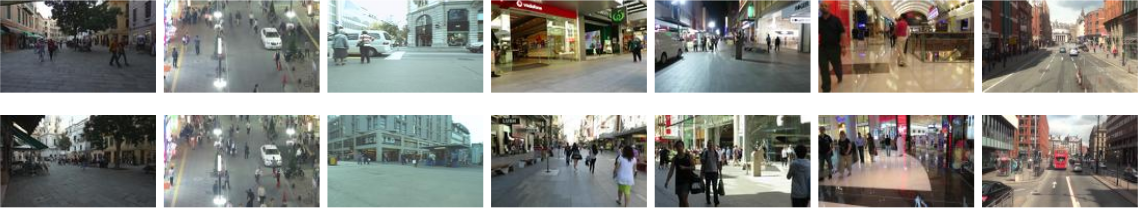
\includegraphics[scale=0.3]{mot16.png}
\caption{An overview of the MOT16 dataset. Top: Training sequences; bottom: test sequences ~\cite{milan2016mot16}}
\label{fig:mot}
\end{center}
\end{figure}
\item \textbf{ALOV}\footnote{{\href{http://alov300pp.joomlafree.it/dataset-resources.html}{ALOV Dataset}}}\\
The Amsterdam Library of Ordinary Videos for tracking is another well-known visual object tracking dataset in the field. It aims to cover as diverse circumstances as possible including illuminations, transparency, zoom or low contrast, for example. The dataset consists of 315 video sequences mainly obtained from YouTube with 64 different types of targets. The sequences are normally short with an average length of 9.2 seconds and the total number of frames is 89364 (in ALOV300).
\item \textbf{CAVIAR} \cite{dubuisson2016survey}\\
The CAVIAR project (Context Aware Vision using Image-based Active Recognition) from INRIA labs was dedicated to the development of algorithms that can describe and understand video scenes. The scenes were associated with surveillance scenarios where people performed some different activities related with the surveillance area. Those activities included \textit{walking}, \textit{browsing}, \textit{resting}, \textit{leaving bags behind} or \textit{two people fighting}. The annotations contain, apart from the bounding boxes locations, the head and feet positions, the body direction, among others. Refering to the tracking task, the challenging problems include occlusions, appearance/disappearance, appearance changing or similar object tracking, for example. In terms of data size, the first set contains 28 video sequences and the second set contains 44 video sequences (Figure \ref{fig:caviar}). It is a well-known dataset and is commonly used for development and testing of tracking algorithms.
\begin{figure}[h!]
\begin{center}
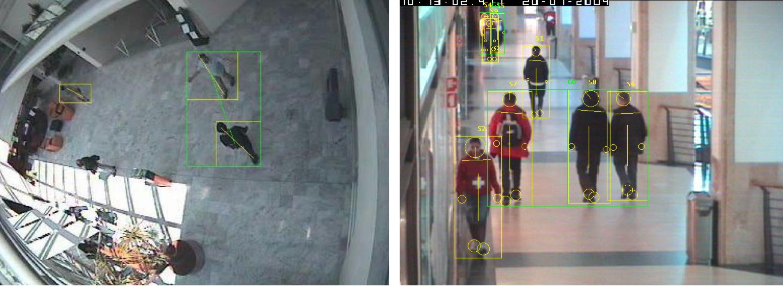
\includegraphics[scale=0.3]{caviar.png}
\caption{CAVIAR: From  left  to right, two frames (ground truth superposed) from sequences of datasets 1 (entrance lobby of INRIA Labs) and 2 (hallway of a shopping center) ~\cite{dubuisson2016survey}}
\label{fig:caviar}
\end{center}
\end{figure}
\item \textbf{BEHAVE} \cite{dubuisson2016survey}\\
Similarly to CAVIAR dataset, the BEHAVE Interactions Test Case Scenarios dataset contains various video sequences with different scenarios where people perform different interactions among which are \textit{walk together}, \textit{meet} or \textit{split} (Figure \ref{fig:behave}). The annotations include labels in case of interactions. Proposed for behavior analysis of interacing groups, this dataset was also used to validate visual for other purposes like the validation of visual tracking algorithms that consider occlusions or fast and varying motion of objects.
\begin{figure}[h!]
\begin{center}
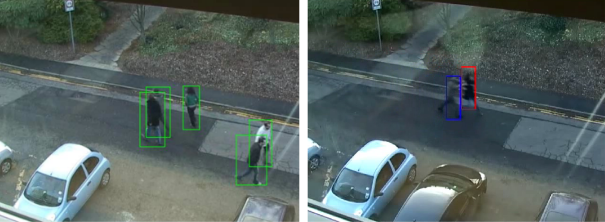
\includegraphics[scale=0.38]{behave.png}
\caption{BEHAVE: Two snapshots of sequences, with the ground truth bounding boxes of the objects to track \cite{dubuisson2016survey}}
\label{fig:behave}
\end{center}
\end{figure}
\item \textbf{PETS} \cite{dubuisson2016survey}\\
The International Workshop on Performance Evaluation of Tracking and Surveillance organizes a visual tracking competition with different objectives on every edition starting from 2000. In 2013\footnote {\href{http://www.cvg.reading.ac.uk/PETS2013/index.html}{PETS 2013}}, two of the objectives were the tracking and counting of people in crowds to estimate the density, and detecting events by crowd analysis. As BEHAVE or CAVIAR, PETS datasets are very popular among the computer vision community. The latest PETS edition took place in 2017\footnote {\href{http://openaccess.thecvf.com/content_cvpr_2017_workshops/w34/papers/Patino_PETS_2017_Dataset_CVPR_2017_paper.pdf}{PETS 2017}} and continued the evaluation theme of on-board surveillance systems for protection of mobile critical assets started in PETS 2016 \cite{patino2016pets}. On this edition, the dataset included sequences that adressed the protection of trucks (Figure \ref{fig:pets}) or vessels at sea, among others.
\begin{figure}[h!]
\begin{center}
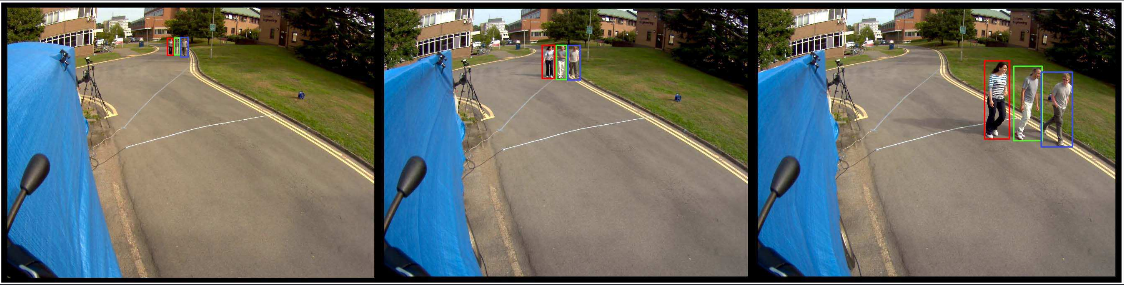
\includegraphics[scale=0.27]{pets2016.png}
\caption{PETS 2016: A group of people detected and tracked walking by the Truck \cite{patino2016pets}}
\label{fig:pets}
\end{center}
\end{figure}
\item \textbf{TrackingNet} \cite{muller2018trackingnet}\\
Most of the commented datasets are limited by its small size. Even more if they are going to be used by data-hungry trackers based on deep-learning. Currently, this trackers rely on object detection datasets due to the lack of dedicated large-scale tracking datasets. For this reason the authors created TrackingNet, the first large-scale dataset and benchmark for object tracking in the wild. TrackingNet provides a total of 30643 video segments with more than 14 million dense bounding box annotations (Figure \ref{fig:trackingnet}). The contributions of this work include different techniques to generate dense annotations from coarse ones and an extended baseline for state-of-the-art trackers benchmarked on TrackingNet. Referring to the latter, the authors affirm that pretraining deep models on this dataset can improve their performance on other datasets by increasing their metrics by up to 1.7\%.
\begin{figure}[h]
\begin{center}
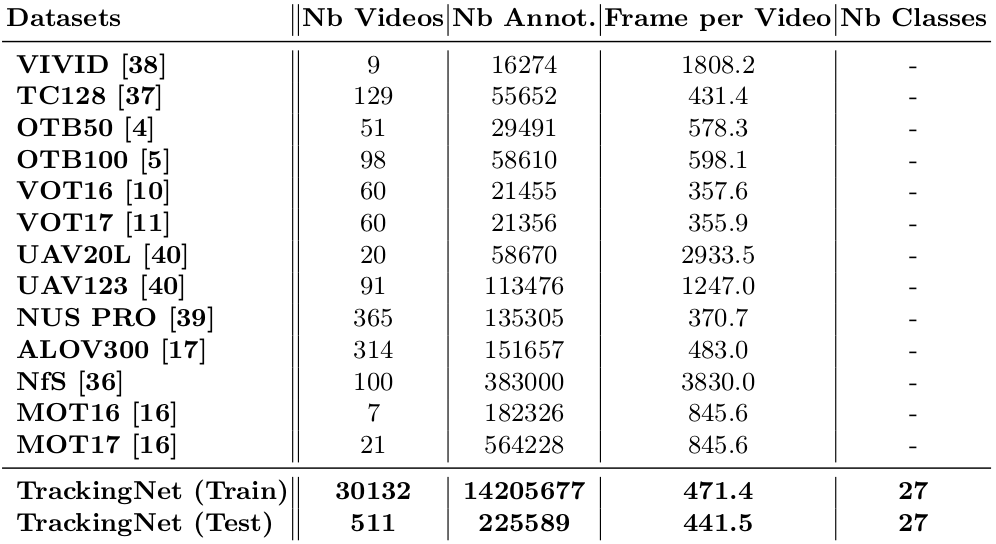
\includegraphics[scale=0.3]{trackingnet.png}
\caption{TrackingNet: Comparison of current datasets for object tracking \cite{muller2018trackingnet}}
\label{fig:trackingnet}
\end{center}
\end{figure}
\end{itemize}

\item \textbf{Single object tracking}
\begin{itemize}
\item \textbf{OTB} ~\cite{wu2013online}\\
As it was said before, for a comprehensive performance evaluation it is critical to collect a representative dataset. There exist several datasets for visual tracking in surveillance escenarios but often the target objects are humans or cars of small size with a static background. Also, some of the scenes are sometimes not annotated with bounding boxes which makes them not very useful for the comparison of tracking algorithms. To facilitate the evaluation task the authors built a tracking dataset with 50 fully annotated sequences in the first release \textit{OTB50}. Later, the dataset was extended with another 50 sequences (\textit{OTB100}).\\ Many factors can affect the tracking performance such as illumination variation or occlussion, for this reason the authors categorized the sequences with 11 attributes according to the occurrence of any of the selected factors (Figure \ref{fig:otb}).\\
\begin{figure}[h!]
\begin{center}
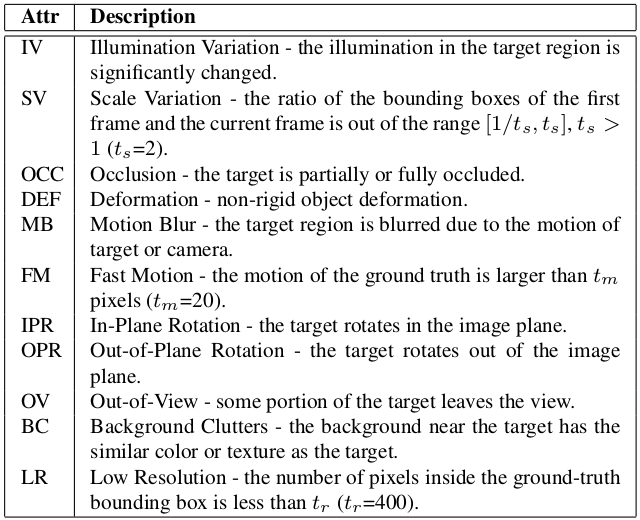
\includegraphics[scale=0.3]{otb_attributes.png}
\caption{OTB: List of the attributes annotated to test sequences ~\cite{wu2013online}}
\label{fig:otb}
\end{center}
\end{figure}
Apart from the data side, the authors also integrated most of the publicly available trackers at the time to create a code library with uniform input and output formats to facilitate large scale performance evaluation. Including TLD \cite{kalal2010pn}, MIL \cite{babenko2009visual} or CPF \cite{perez2002color} making a total of 29 tracking algorithms.
\item \textbf{VOT} \cite{kristan2017visual}\\
The Visual Object Tracking initiative was started in 2013 to address performance evaluation of short-term visual object trackers. The short-term tracking means that trackers are assumed to not be capable of performing successful re-detection after the target is lost and they are therefore reset after such event. In all the previous editions the challenge considers single-camera, single-target, model-free\footnote{The only training information provided is the bounding box in the first frame}, causal trackers\footnote{The tracker does not use any future frames, or frames prior to re-initialization, to infer the object position in the current frame}, applied to short-term tracking. The main goal of VOT is establishing datasets, evaluation measures and toolkits for visual object tracking (as many other initiatives). The successive editions were made in conjunction with Computer Vision Conferences like ICCV or ECCV. In 2015, a subchallenge focussed on tracking in thermal infrared (\textit{TIR}) was made due to the growing interest in this kind of imaging. The 7th Visual Object Tracking Challenge VOT2019 workshop will be held in conjunction with the ICCV2019. With respect to the previous edition in 2018, this challenge edition introduces the evaluation of trackers that use 4 channels (\textit{RGB-IR} and \textit{RGB-depth}).\\
Referring to the data itself, the VOT datasets try to pay more attention to the diversity of the data and the quality of the content and annotation with respect to the quantity. For example, some datasets assign a global attribute to the entire sequence when it is happenning in a fragment of it. VOT dataset tries to avoid the assumption that the quality of the data is correlated with its size. The VOT Challenge has focused on developing a methodology for automatic construction and annotation of moderately large datasets from a  large pool of sequences (Figure \ref{fig:vot}). For example, they use sequences from datasets such as the OTB dataset.
\begin{figure}[h!]
\begin{center}
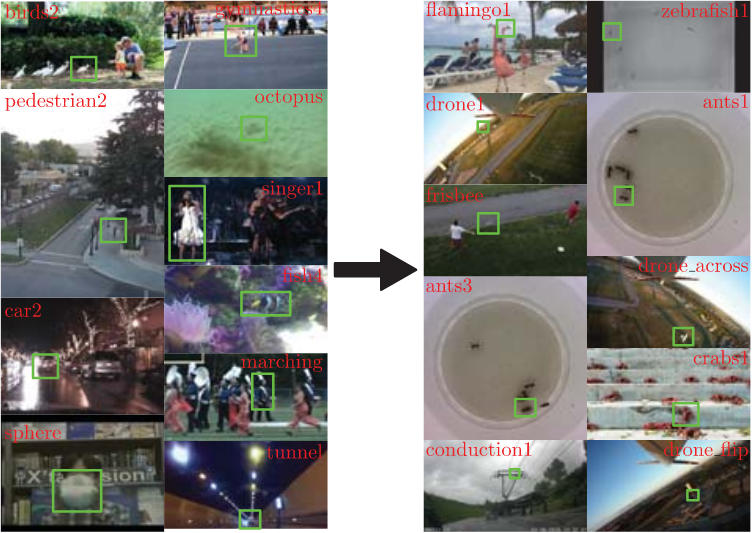
\includegraphics[scale=0.3]{vot.png}
\caption{VOT: Images from the VOT2016 sequences (left column) that were replaced by new sequences in VOT2017 (right column) ~\cite{kristan2017visual}}
\label{fig:vot}
\end{center}
\end{figure}
\item \textbf{Need for Speed} \cite{kiani2017need}\\
Visual object tracking algorithms have been usually evaluated at the canonical frame rate of 30 frames per second (\textit{FPS}) but consumer devices with cameras such as smartphones, tablets or drones are increasingly coming with higher frame rates. This can take time for the visual object track community to adapt to what \textit{real time} means in terms of how faster frame rates affect the choice of a tracking algorithm. The authors introduce Need for Speed (\textit{NfS}) as the first higher frame rate video dataset and benchmark for visual object tracking. The dataset consists of 100 videos captured with 240 FPS cameras from real world scenarios. The frames are annotated with bounding boxes and the sequences are manually labelled with nine visual attributes (occlusion, fast motion, etc.). The work also provide a ranking of many recent state-of-the-art trackers according to their tracking accuracy and real-time performance. One interesting conclusion the authors obtained is that at higher frame rates, simple trackers such as correlation filters outperform complex methods based on deep learning. This must be important when making the choice of a tracking algorithm in practical applications. It needs to be a tradeoff between the resources (available bandwidth, computation hardware, etc.) and the required application accuracy.
\end{itemize}
\end{itemize}
\subsection{Metrics}
%-------------------------------------------------------------------------
\subsection{Previous work on tracking}
Once the bases on which the project is based are seen, it is necessary to see what have been and are the works that form the State of the Art in the techniques that will be used to solve the problem that arises. Therefore, in this section we will talk about object tracking methods.\\ %cambiar
In the field of computer vision there is a wide variety of study areas, one of the most important is the so-called \textit{object tracking}. Its main objective is to estimate the state of the object (\textit{target}) over time in a series of sequences of images (\textit{frames}). This state can be defined by different characteristics such as shape, appearance, position or speed.\\
It is a difficult field since one or more circumstances can be given that must be solved by the algorithm. Among them are the management of variations in lighting and in the point of view of the object that can lead to changes in the appearance of the same. Likewise, the occlusions that occur when objects are mixed with other elements of the scene or the quality of the image itself may be a problem to consider in this area.\\
To confront these problems the following paradigms have been followed ~\cite{smeulders2014visual}:
\begin{itemize}
\item \textbf{Tracking using matching}: this group of algorithms makes a \textit {matching} between the representation of the model of the object created from the previous frame and the possible candidates in the next frame. The most outstanding methods are \textit{Normalized Cross-Correlation} ~\cite{briechle2001template}, \textit{Lucas-Kanade Tracker} ~\cite {baker2004lucas}, \textit{Kalman Appearance Tracker} ~\cite{nguyen2004fast} and \textit{Mean Shift Tracking} ~\cite{comaniciu2000real}.
\item \textbf{Tracking-by-detection}: a model is built to distinguish the object from the background ~\cite{nguyen2006robust}. Once you have the detection it is associated with the other detections. Currently, the community is turning to neural networks to compute detections.
\item \textbf{Tracking, learning and detection}: it is an extension of the previous group that includes a mechanism to update the model that is learned during execution. For example, you can use the results of a \textit{optical flow tracker} for this update ~\cite{kalal2010pn}. This ensures that the algorithm is invariant to changes in the object. 
\end{itemize}
Prior to the modern techniques to be discussed there are more classic ways of tracking objects that can be useful in problems that require real time when tracking, for example. One of the best known is \textit{feature tracking}. This technique uses characteristic points that can be found in the images and that allow to estimate the movement. These points must meet some requirements to be able to be characteristic of the image such as repeatability (the characteristic can be found in the images even if they have undergone some transformation), compatibility (each characteristic must be descriptive and easy to find) or efficiency (the representation of the information characteristic of the image must be done with as few characteristics as possible). Some of the characteristic points most commonly used are corners. They are characterized by gradients with higher values in them in two or more directions. These techniques include Harris ~\cite{harris1988combined} and Shi-Tomasi corner detectors ~\cite{shi1994good}.\\
There are tracking systems that take advantage of the speed of feature tracking and the accuracy of neural networks to create a hybrid tracking. In this type of tracking the detections are done each N frames using some type of neural network and the intermediate tracking is done through feature tracking.\\
With the arrival of neural networks this way of grouping the different tracking methods changes to adapt to them ~\cite{held2016learning}:
\begin{itemize}
\item \textbf{Tracking-by-detection}: they are designed to follow a certain class of object (\textit{model-based}) and to obtain a specific classifier. In the test phase the detections obtained with neural networks are linked using temporal information. They are limited to a single class of objects.
\item \textbf{Tracking, learning and detection}: they are characterized by being fully trained \textit{online}. A typical tracker example of this group samples zones close to the object and considers them "\textit{foreground}", the same happens with the distant zones that would be assigned to the "\textit{background}". With this you can build a classifier that differentiates them and estimate the new location of the object in the following frame ~\cite{babenko2009visual}. It has been tried to introduce neural networks in environments with online training but due to the slowness of the networks when training the results are slow in test phase.
\item \textbf{Siamese-based tracking}: this type of networks use \textit{patch-matching} techniques ~\cite{tao2016siamese}.   Multiple patch candidates from the new frame are received and the one with the highest \textit{matching score} with respect to the previous frame is chosen as the best candidate, that is, the most similar according to the matching function.
\item \textbf{Tracking as regression}: in this group, on the other hand, the network receives only two images and directly returns the location of the object ~\cite{held2016learning}.
\item \textbf{Tracking con RNN}: from the detection obtained this type of algorithms use \textit{Recurrent Neural Networks} to model the sequence of movement of objects thus improving the response to prolonged occlusions in time, for example ~\cite{sadeghian2017tracking}. They are the state of the art in tracking today. %revisar
\end{itemize}


\lhead[]{CHAPTER \thechapter. Software infraestructure}
\chapter{Software infraestructure}

For the use of Deep Learning have emerged numerous \textit{frameworks}. A deep learning framework allows us to build deep learning models more easily and quickly, without getting into all the details of the underlying algorithms. These are some of the most used today:
\begin{itemize}
\item \textbf{Tensorflow}: ofrece un API de bajo nivel que permite un control completo sobre los diseños de los modelos y también un API de alto nivel más simplificado pero con una funcionalidad limitada. Además permite la visualización del entrenamiento mediante la herramienta Tensorboard.
\item \textbf{Keras}: proporciona un API de alto nivel para uso de redes de neuronas. Puede correr sobre distintos \textit{backends} como Theano o Tensorflow y dispone modelos de redes pre-entrenadas que permiten crear una red de forma sencilla. Escrita en Python, ofrece un entorno amigable y modular.
\item \textbf{Caffe}: emplea una arquitectura C++/CUDA optimizada para uso en GPU y proporciona interfaces para Python o Matlab, por ejemplo. La definición del modelo se hace mediante Protobuf, formato creado por Google, creando una estructura de datos serializada. También dispone de modelos pre-entrenados e interfaz gráfico.
\item \textbf{PyTorch}:
\end{itemize}

\lhead[]{CHAPTER \thechapter. Multiobject tracking using deep learning and tracking by detection}
\chapter{Multiobject tracking using deep learning and tracking by detection}
In this chapter, the solution obtained for solving the multiobject tracking problem using deep learning and tracking-by-detection is explained.

\section{Design overview}
The main contribution of this work is to develop a tracking algorithm capable of tracking different types of objects using deep learning techniques. To achieve this task the selected tracking methodology is the tracking by detection. Our method combines detections coming from an object detection neural network with tracking techniques. With this, the idea is to give the final system a balance between speed and accuracy. The detections from the neural networks are usually slower than a pure tracking but more accuracted whereas the tracker results are often quickly obtained but they are slightly more inaccurated.\\
The module architecture of the system is summarized in the following diagram (Figure \ref{fig:general}).
\begin{figure}[H]
\begin{center}
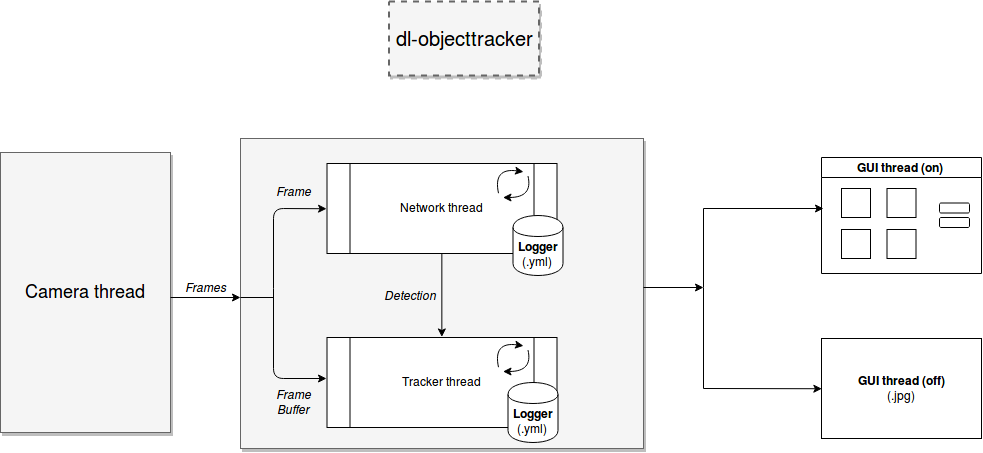
\includegraphics[scale=0.4]{figures/general.png}
\caption{modular architecture}
\label{fig:general}
\end{center}
\end{figure}

As it can be seen the system is built in a modularized way with different threads. There are 4 threads: Camera, GUI, Network and Tracker. All of them are going to be discussed more in deep on its respective sections of the chapter but the general workflow of the system is going to be explained here (Figure \ref{fig:update_cam}).\\
First, the camera thread provides the images or frames to the rest of the threads, i.e.\ the input to the system. The output of the system can be provided using an YML file with the results per frame (\textit{Logger}) or using the GUI. If the GUI is configured to show the graphical interface (\textit{on}), the results are shown on screen. But if the graphical interface is not configured (\textit{off}) the results are saved in JPG files.\\ The core of the computing is divided in the Network thread and the Tracker thread. This Tracker has a buffer of frames of different size coming from the Camera to work on \textit{delayed real-time}. So, when the first frame is available it is given to the Network thread which starts doing the inference, this is, it starts detecting objects. Meanwhile, the buffer is accumulating the incoming frames from the Camera until the detection from the Network comes.\\
When the detection is available, the Tracker thread starts the tracking of the detected objects in the buffer of frames. The last frame in the buffer is used to feed again the Network allowing for a synchronism between the detections and the tracking in the frames. This temporal process can be observed more clearly in the Figure \ref{fig:buffer}.
\begin{figure}[H]
\begin{center}
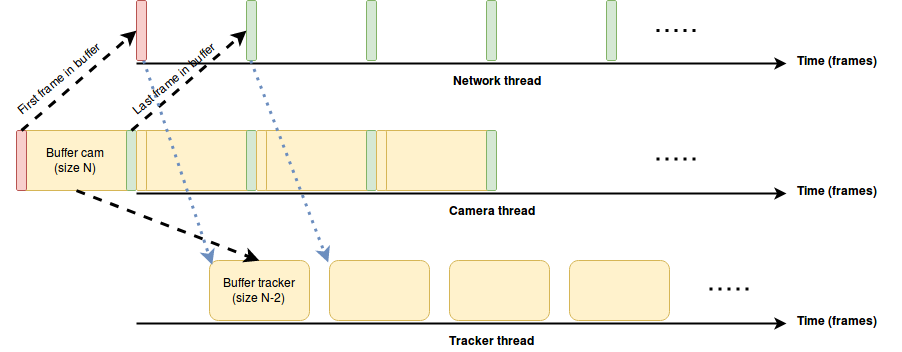
\includegraphics[scale=0.4]{figures/buffer.png}
\caption{How the buffer is handled}
\label{fig:buffer}
\end{center}
\end{figure}
It can be seen that given a complete buffer in Camera of size \textit{N}, the first frame is assigned to the Network and, when this frame is processed, a buffer of size \textit{N-2} is assigned to the Tracker to be processed. The last frame of the given buffer is passed to the Network again. This iterative mechanism continues in time ensuring that no frames are lost. The application has always a delay in frames of 1 buffer (\textit{delayed real-time}).
\\As commented before, the buffer changes its size in every iteration but we can not allow the buffer to increase or decrease this size in an uncontrolled way because that will end blocking the system. If the buffer is too big, the tracking will take more time and the neural network will finish before the tracking is done. This is, the Network is underused. In the other side, if the buffer is too small, the Tracker will end its work before the inference is done in the Network and the Tracker will have to wait much more time to the Network to finish. For these reasons a balance is needed.\\
The neural network inference time is approximately the same time so this time is fixed. Then, the only part of this processing core where we can change is on the Tracker side. The obtained solution consists of a Tracker which constantly measures its frame rate (FPS) allowing it to slow down or speed up depending on this measurement.\\
Once all the frames have been processed the Network and Tracker thread stop. After that, the results are logged into the YML files (a file for each frame) and the user can close the application.\\
The general behavior of the application when running video sequences or raw frames was presented. Nevertheless, it can also handle live stream videos coming from local cameras connected. In this case, the logging of the results is not done but the tracking by detection scheme is the same.\\
The ``main" is done in the \texttt{update} function of the Camera which is continuously called by the Camera thread. As the system architecture is based in multiple threads, the synchronism between them is crucial. Because of this, the control of the application is done taking into account the synchronism between all the threads, their internal status and variables.
\begin{figure}[H]
\begin{center}
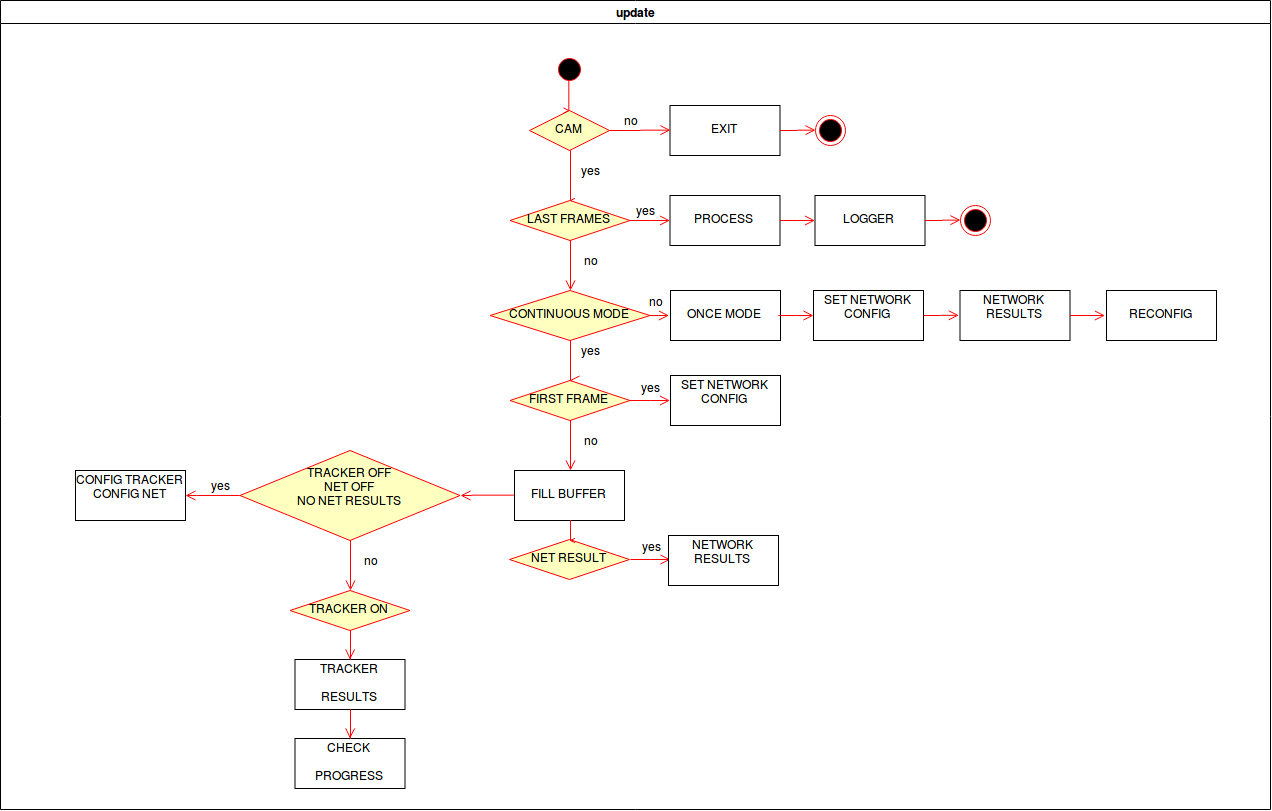
\includegraphics[scale=0.3]{figures/update_camera.png}
\caption{The control flow}
\label{fig:update_cam}
\end{center}
\end{figure} 

As commented in the chapter 2, the application is configurable using an YML file (\textit{objecttracker.yml}). For the instructions on how to run the application please refer to the wiki of the project (see \ref{Methodology}).
\\In the next sections, the implementation of each thread of the system is explained, including the available configuration modifications.\\

\section{Video source}
The Camera module provides the input images to the rest of the system. This images can be obtained using four different sources:
\begin{itemize}
    \item \textbf{Local camera (with OpenCV)}: the Camera can read from a local camera using the OpenCV routine \texttt{VideoCapture} indicating the device number of the camera.
    \item \textbf{Local camera (with ROS)}: the Camera can use ROS to read from the camera device. In order to do so, the user needs to launch a terminal and type \texttt{roslaunch usb\_cam.launch}. This will publish a ROS topic \texttt{/usb\_cam/image\_raw} that can be subscribed by the Camera module and it will start reading frames from the device. For more information about the launching process please refer to my wiki (\ref{using_ros}).
    \item \textbf{Local video}: to read from a local video it is also used the OpenCV routine \texttt{VideoCapture} but indicating the video path.
\item \textbf{Local images}: similarly the local images path needs to be passed to \texttt{VideoCapture}. This source is very useful because most of the datasets are provided as sequences of frames instead of videos. And it can avoid problems such as creating sequences of videos with the wrong duration or frame rate.
\end{itemize}
The Camera thread source and options can be modified at the configuration file. The source is selected at \texttt{ObjectTracker->Source}. After that the user needs to indicate the device number \texttt{ObjectTracker->Local->DeviceNo} if using a local camera with OpenCV, the video path \texttt{ObjectTracker->Video->Path} if using a local video or the images path \texttt{ObjectTracker->Images->Path} when using local images.\\
The user needs to modify the \texttt{usb\_cam.launch} to change the Camera configuration when using ROS.\\
Before being sent to other threads the image is rescaled according to the neural network input size. It continues all the process with this size. When the final results are obtained this is taken into account to rescale the coordinates of the detections or trackers with respect to the original image size.\\
Apart from providing images the Camera thread also controls the flow of the application. This is done in this way because the application offers the option of not having GUI. In the first versions of the project the control of the application (the ``main") was implemented in the GUI thread but when the no-GUI option was added this was moved to the Camera thread.\\

\section{GUI}
The GUI module provides the interface with the user and, as commented before, is optional. It was implemented using the tools provided by PyQt5, in concrete with the packages \textit{QtGui, QtCore} and \textit{QtWidgets}.\\
The graphical interface has four windows and two buttons. The top-left window shows the input frames in real-time while the top-right one shows the final results. The intermediate results obtained from the Network and the Tracker will be provided at the bottom. The application with GUI has two modes with its respective buttons: ``run continuous" and ``run now". In the first one, the application runs continuously until it finishes the process (the process finishes depending on the image source). In the second one, the user can push the \textit{Run now} button to make the Network detect on the current frame and continue the tracking from that frame towards.
\section{Neural Network} 
The Network module is tasked with the object detections in the images which are feeding the Tracker on every iteration. It supports Tensorflow and Keras object detection models. The Tensorflow models can be obtained from the Tensorflow detection model zoo\footnote{\href {https://github.com/tensorflow/models/blob/master/research/object_detection/g3doc/detection_model_zoo.md}{Tensorflow detection model zoo}} and include SSD and R-CNN detectors. The Keras models are limited to SSD architectures and it can be obtained from this set\footnote{\href {https://github.com/pierluigiferrari/ssd_keras#download-the-original-trained-model-weights}{Keras models}}.\\
The datasets on which the model was trained need to be specified to assign the labels to the objects. The supported labels include the VOC, COCO, KITTI, OID and PET datasets. As it ocurred with the Camera module the Network module has configurable options available in \textit{objecttracker.yml}:
\begin{itemize}
    \item \texttt{Framework}: Keras or Tensorflow
    \item \texttt{Model}: the model file
    \item \texttt{Dataset}: VOC/COCO/KITTI/OID/PET
    \item \texttt{Input size}: this input size can be modified depending on the selected model. Some models does not allow to change the input image size
    \item \texttt{Confidence}: the confidence threshold for the detections obtained. If a detection obtains a confidence value below that detection is discarded
\end{itemize}
The Network thread basically receives an image (previously resized) and performs the inference. As a result it outputs the detections obtained in the image (if any) and it draws these detections in form of bounding boxes containing also the label and the confidence value.\\
The logging of the Network and Tracker results are optional and it can be changed at the YML configuration file in \texttt{ObjectTracker->Logger->Status}. These results are logged in the \texttt{logNetwork} and \texttt{logTracker} functions respectively.\\

\subsection{Tensorflow models}
These models are obtained from the Tensorflow detection model zoo which provides models for inference out-of-the-box, i.e.\ to be directly used. From the models available only some of them were tested for its use in the project. The pre-trained models used were trained on the COCO dataset because the classes available in this dataset were considered enough for the type of objects that can be seen in the tracking sequences used. In the next table, the Tensorflow models performance can be seen:
\begin{table}[H]
\begin{center}
\begin{tabular}{|c|c|c|}
\hline
Model name                                 & Speed (FPS) & COCO mAP \\ \hline
\textbf{ssd\_mobilenet\_v2\_coco}          & 32         & 22       \\ \hline
\textbf{faster\_rcnn\_inception\_v2\_coco} & 17         & 28       \\ \hline
\textbf{mask\_rcnn\_inception\_v2\_coco}   & 13         & 25       \\ \hline
\end{tabular}
\end{center}
\caption{Tensorflow models performance (from \href{https://github.com/tensorflow/models/blob/master/research/object_detection/g3doc/detection_model_zoo.md#coco-trained-models}{Tensorflow detection model zoo}). Note: the COCO mAP numbers here are evaluated on COCO 14 minival set using the \href{http://cocodataset.org/#detection-eval}{MSCOCO evaluation protocol}}
\end{table}
The reported running time in ms is done for 600x600 images (including all pre and post-processing). As the authors say, ``these timings depend highly on one's specific hardware configuration (performed using an Nvidia GeForce GTX TITAN X card) and should be treated more as relative timings in many cases". However, some characteristics of each model can be extracted in terms of speed and accuracy. As expected, the R-CNN models achieve better accuracy while performing a little slower with respect to SSD.

\subsubsection{SSD MobileNetV2}
This SSD implementation uses MobileNetV2 as backbone. As commented in \ref{mobilenet}, MobileNetV2 is a network proposed to work on mobile devices, this can be interesting to the project because of the hardware limits (it needs to work on CPU only).
\subsubsection{Faster R-CNN InceptionV2}
This region-based model was discussed in \ref{mobilenet}. The implementation uses InceptionV2 \cite{szegedy2016rethinking} as the feature extractor. This backbone follows the idea of its predecesor (InceptionV1) and adds two main ideas: reduce the representational bottleneck and use smart factorization methods. Refering to the first one, the intuition is that neural networks usually perform better when the convolutions do not alter the dimensions of the input in a drastical way (may cause loss of information). To solve this problem they expand the inception module making it wider (instead of deeper). Apart from that, the convolutions are made more efficient in terms of computational complexity. The authors propose factorizing the 5x5 convolution into two 3x3 convolution operations making it 2,78 times faster, among others.
\subsubsection{Mask R-CNN InceptionV2}
This state-of-the-art instance segmentation network is used as object detection network because it offers the bounding boxes locations, apart from the instance masks (Figure \ref{fig:maskrcnn_tests}). The implementation selected also makes use of InceptionV2 behind Mask R-CNN.
\begin{figure}[H]
\begin{center}
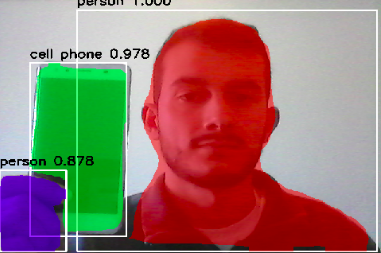
\includegraphics[scale=0.5]{figures/maskrcnn_first_tests.png}
\caption{First tests with Mask R-CNN using live video}
\label{fig:maskrcnn_tests}
\end{center}
\end{figure} 
\subsection{Keras models}
The Keras network is a Keras port of the SSD model architecture introduced by Wei Liu et al. in \cite{liu2016ssd} from SSD-Keras\footnote{\href{https://github.com/pierluigiferrari/ssd_keras}{SSD Keras}}. The repository offers pre-trained models and allows the model training from scratch. The base network architecture used is VGG (see \ref{mobilenet}). The pre-trained models used were trained on the PASCAL VOC dataset. The pre-trained models available include COCO and ILSVRC datasets but PASCAL was selected because COCO dataset was already used in the previous SSD model in Tensorflow. In the next table, it can be seen the reported performance made by the author:
\begin{table}[H]
\begin{center}
\begin{tabular}{|c|c|c|}
\hline
Model name               & Speed (FPS) & VOC2007 test mAP @ 0,5 \\ \hline
\textbf{SSD300\_VOC0712} & 39          & 77,5                   \\ \hline
\textbf{SSD500\_VOC0712} & 20          & 79,8                   \\ \hline
\end{tabular}
\end{center}
\caption{Keras models performance (from \href{https://github.com/pierluigiferrari/ssd_keras#performance}{SSD-Keras performance}). Note: evaluated using official Pascal VOC 2012 test server using an NVIDIA GeForce GTX 1070 mobile.}
\end{table}
The author affirms that the implementation performs slightly better than the original SSD implementation in Caffe\footnote{\href{https://github.com/weiliu89/caffe/tree/ssd}{SSD-Caffe}}.

\section{Tracker}
The Tracker module is the core of the project and therefore it is going to be explained more in deep.\\
As previously commented, the Tracker receives an input detection coming from the Network module and performs the multiobject tracking over a buffer of variable size following a tracking by detection scheme. With this hybrid tracker it is pretended to show the advantages of the tracking by detection with deep learning over a pure neural network tracking or a classic feature tracking.\\
The tracker can work in three operating regimes: \textit{slow, normal} and \textit{fast}. The calculation of this regime is performed using an internal buffer of FPS rates of size 3. The length selected is due to the fact that the tracker needs to respond quickly to changes in its velocity avoiding slowing down or speeding up in an excessive way. The tracker speed calculation is explained in Algorithm \ref{tracker_speed}. Three frame rate thresholds are established to distinguish between a tracker which is behaving in a normal way or a slower or a faster processing time. If the tracker is performing slower than normal the next three frames that needed to be tracked are discarded from the buffer in the \texttt{imageToTrack} function. In the other hand, if the tracker is going too fast it is slowed down in \texttt{getOutputImage} by waiting some frames to return the image to be output. With this mechanism the buffer does not increase or decrease too much in size allowing a more stable behavior and a good synchronization between the threads.

\begin{algorithmic}[H]
\begin{algorithm}
\State \textbf{Inputs:} averageFPS, lastFPSBuffer, trackerSlow, trackerFast, counterSlow, counterFast
\State \textbf{Output:} trackerSpeedMode
\Procedure{trackerSpeedMode}{}
\If {not 0 in $lastFPSBuffer$ and $averageFPS$ \textless 10}
    \State $counterSlow$ + 1
    \If {$counterSlow$ == 3}
        \State $counterSlow$ = 0
        \State $trackerSlow$ = True
    \EndIf
\ElsIf{not 0 in $lastFPSBuffer$ and 10 \textless $averageFPS$ \textless 25}
    \State $trackerSlow$ = False
    \State $trackerFast$ = False
\ElsIf{$averageFPS$ \textgreater 25 and $counterFast$ \textless 1}
    \State $counterFast$ + 1
\State $trackerFast$ = True
\EndIf  
\EndProcedure
\caption{Tracker speed mode}\label{tracker_speed}
\end{algorithm}
\end{algorithmic}

This dynamic calculation allows the tracking to behave differently depending on the operating regime in which it is on each instant. However, it will be seen in the next chapter that this regime is very depending on the tracker that is being used and its speed performance.\\
The tracking will be performed using already built tracking implementations of two libraries: OpenCV and dlib. This will also allow for a good comparative between them that can lead us to select the preferred option for the tracking algorithm. In the next subsection, the tested tracker implementations are discussed.
\subsection{OpenCV tracking}
OpenCV is known for the great variety of algorithms for which it provides implemented solutions, one of them is tracking. This libraries are included in the OpenCV extra modules (\texttt{opencv contrib}).\\
The tested trackers include \textit{BOOSTING, MIL, MEDIANFLOW, TLD, KCF, MOSSE} and \textit{CSRT} (in release order).
\\
The OpenCV trackers available in this project are now introduced:
\begin{itemize}
\item BOOSTING \cite{grabner2006real}: based on an online version of AdaBoost, the tracker is trained at runtime with positive and negative examples of the object to track. An initial bounding box needs to be provided by the user or other object detection algorithm. The classifier looks over the pixel neighborhood of a previous location to find the new location. The classifier is constantly updated with this new positives.
\item MIL \cite{babenko2009visual}: the \textit{Multiple Instance Learning} algorithm tries to solve the problem of learning an adaptive appearance model for object tracking. To achieve this, the authors train a discriminative classifier online to separate the object to track from the background, i.e.\ positive and negative examples are extracted from the frame (Figure \ref{fig:mil}). Similarly to the Boosting algorithm, the model searches inside of the window of the old location. It obtains a probability map with most probably new location of the object and updates the tracker model.
\begin{figure}[H]
\begin{center}
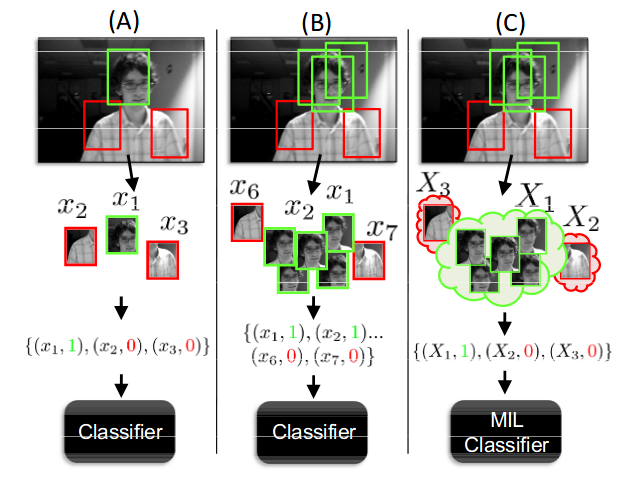
\includegraphics[scale=0.4]{figures/mil.png}
\caption{Updating a discriminative appearance model: (A) using a single positive image patch. (B) using several positive image patches. (C) using one positive bag of several image patches (from \cite{babenko2009visual})}
\label{fig:mil}
\end{center}
\end{figure}
\item MEDIANFLOW \cite{kalal2010forward}: the Median Flow algorithm introduced a novel method for tracking failure detection based on the Forward-Backward error. This  basically consists of perform the tracking forward and backward in time in a given frame and measure the discrepances between trajectories (see Figure \ref{fig:medianflow}). The authors affirm that this discrepances are highly correlated with real tracking failures.
\begin{figure}[H]
\begin{center}
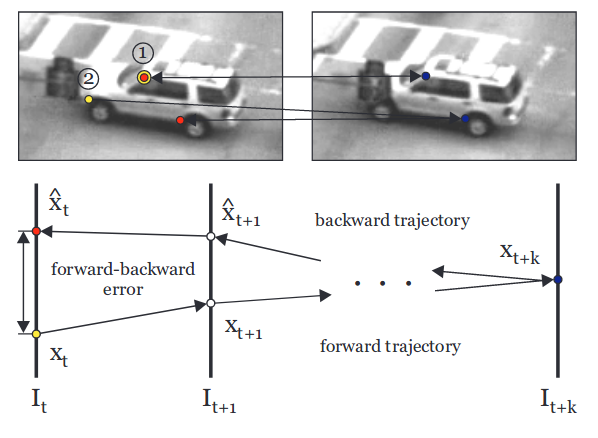
\includegraphics[scale=0.4]{figures/medianflow.png}
\caption{The forward-backward error in Point 2 (from \cite{kalal2010forward})}
\label{fig:medianflow}
\end{center}
\end{figure}    
\item TLD \cite{kalal2011tracking}: in the original paper on which is based the implementation, the authors investigate the long-term object tracking and propose a novel framework that descompose this type of tracking into \textit{tracking, learning and detection} (TLD). The tracker based on Median Flow follows the object in every frame. The detector is composed by a patch variance module, followed by an ensemble classifier and finally a Nearest Neighbor classifier. The function of this detector is to correct the tracker if necessary. The learning step estimates the errors of the detector and updates it using a novel method called \textit{P-N learning}.
\item KCF \cite{henriques2012exploiting}: the \textit{Kernelized Correlation Filter} is a tracking framework that utilizes properties of circulant matrix to enhance the processing speed. The authors observed that the translated and scaled patches used to train discriminative classifiers contain redundancies and the resulting data matrix from this patches is circulant. With kernel regression as classification method they derive the KCF tracking.
\item MOSSE \cite{bolme2010visual}: correlation filters can track complex objects in common tracking scenarios that may include rotations, occlusions or other distractions at high frame rates. The \textit{Minimum Output Sum of Squared Error} filter is another type of correlation filter. Filter based trackers model the appearance of objects using filters trained in example images (Figure \ref{fig:mosse}). With a given initial target in the first frame the tracking and the filter training start to work together. The idea behind MOSSE is an optimization problem, given a set of training images $f_i$ and training outputs $g_i$, MOSSE finds a filter \textit{H} that minimizes the sum of squared error between the actual output of the convolution and the desired output of the convolution (see Formula \ref{eq:conv_mosse}).
\begin{equation}
\min_{H^*}\sum_{i}\left|F_i \odot H^* - G_i\right|^2
\label{eq:conv_mosse}
\end{equation}

\begin{figure}[H]
\begin{center}
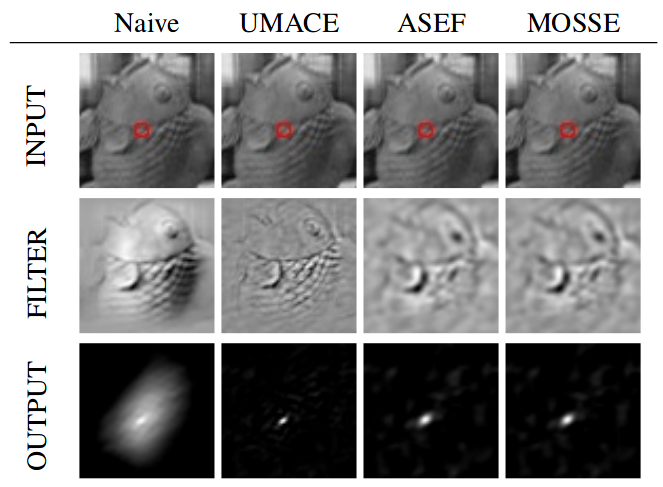
\includegraphics[scale=0.35]{figures/mosse_filter.png}
\caption{Comparison of the output peaks produced by different correlation filters (from \cite{bolme2010visual})}
\label{fig:mosse}
\end{center}
\end{figure} 

\item CSRT \cite{lukezic2017discriminative}: the CSRT tracker is based on the paper \textit{Discriminative Correlation Filter with Channel and Spatial Reliability}. Here the authors introduce the channel and spatial reliability concepts to DCF tracking to improve the filter update and the tracking process (Figure \ref{fig:csrt}). The spatial information is used to restrict the searching to the parts suitable for tracking. In the other hand, the channel information aims to reduce the noise of the weighted-averaged filter response.
\begin{figure}[H]
\begin{center}
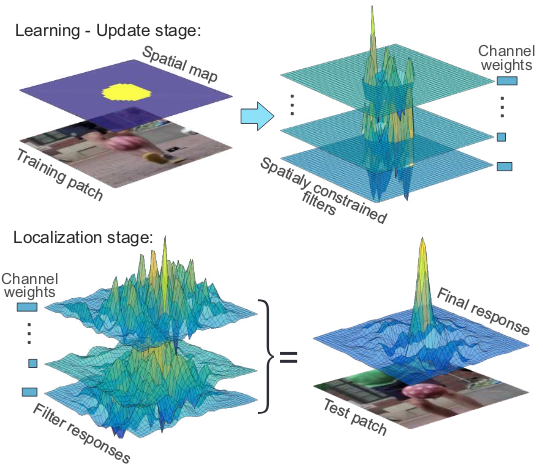
\includegraphics[scale=0.4]{figures/csrt.png}
\caption{Overview of the CSR-DCF approach (from \cite{lukezic2017discriminative})}
\label{fig:csrt}
\end{center}
\end{figure} 
\end{itemize}

In the next chapter, some experiments are performed to put into practice the advantages and disadvantages of each OpenCV tracker. Furthermore, the dlib tracking will also be discussed allowing for a comparison between all the proposals and allowing us to select the best tracker option.
\subsection{dlib tracking}
In chapter 2, the dlib library was introduced as a set of independent software components that provide different utilities, one of them is tracking. The \texttt{dlib.correlation\_tracker} is going to be used for this project. As the name indicates, it is another implementation of a correlation filter for tracking which are widely used. This tool is an implementation of the method described in \cite{danelljan2014accurate}.\\ In the proposed solution, the authors are centered in solving the challenging problem of handling large scale variations in visual object tracking. They propose a method for a robust scale estimation in a tracking by detection framework, as it is the case in this project. To do so the learning of discriminative correlation filters is based on a scale pyramid representation.


\lhead[]{CHAPTER \thechapter. Experiments}
\chapter{Experiments}
In this chapter, the quality of the Network and Tracker modules is characterized. First, the available neural networks will be evaluated with a common tracker to select the final neural network used in the dl-objecttracker application. Second, several trackers implementations will be also characterized using the selected neural network. The configurable parameters will be adjusted to select the best performing values. This will give us the best combination of Network and Tracker modules for the final dl-objecttracker, which will also be experimentally validated.\\
\section{Experimental setup}
The experiments were performed on a laptop PC with \textit{Intel® Core™ i7-4510U CPU @ 2.00GHz x 4} and no GPU acceleration.\\ As commented in section \ref{metrics_tool}, the Object Detection Metrics tool was used to compute the following metrics: precision, recall and AP. It is necessary to mention that the tool was slightly modified to provide the TP, FP and GT numbers. The speed measuremenents are obtained directly from the \texttt{dl-objecttracker} for both the Network and the Tracker modules.\\
The selected dataset for evaluating the tracking application and its modules is the MOT17Det \cite{milan2016mot16} \textit{train} set (see Table \ref{tab:annex_3}). The results were not evaluated on the \textit{test} set due to the fact that the official web of the challenge does not include in the provided data the annotated ground truth of the test set. To obtain the ground truth from this dataset and adapt it to the metrics tool a small Python script was developed in this project following the official reference \cite{milan2016mot16}. However, some modifications were done to allow the compatibility between the metrics tool and the labels of the detections (the neural networks are trained in COCO or PASCAL) (see Table \ref{tab:mot_labels}). Following the official MOT interpretation of ground truth detection files, the final ground truth obtained from the train set only includes the \textit{person} class.
\begin{table}[H]
\scriptsize
\begin{center}
\begin{tabular}{|c|l|l|}
\hline
\textbf{ID}                       & \multicolumn{1}{c|}{\textbf{Label in MOT gt}} & \multicolumn{1}{c|}{\textbf{Label in our gt}} \\ \hline
\textbf{1}                        & Pedestrian                                    & Person                                        \\ \hline
\textbf{2}                        & Person on vehicle                             & Car                                           \\ \hline
\textbf{3}                        & Car                                           & Car                                           \\ \hline
\textbf{4}                        & Bicycle                                       & Bicycle                                       \\ \hline
\textbf{5}                        & Motorbike                                     & Motorbike                                     \\ \hline
\textbf{6}                        & Non motorized vehicle                         & Bicycle                                       \\ \hline
\textbf{7}                        & Static person                                 & Person                                        \\ \hline
\textbf{8}                        & Distractor                                    & -                                             \\ \hline
\textbf{9}                        & Occluder                                      & -                                             \\ \hline
\textbf{10}                       & Occluder on the ground                        & -                                             \\ \hline
\textbf{11}                       & Occluder full                                 & -                                             \\ \hline
\multicolumn{1}{|l|}{\textbf{12}} & Reflection                                    & -                                             \\ \hline
\end{tabular}
\end{center}
\caption{Label equivalences with MOT ground truth in our ground truth}
\label{tab:mot_labels}
\end{table}
\section{Neural network selection}
The correct selection of a neural network model for object detection is crucial in this project as it provides the previous detections the tracker module needs to track. As commented in section \ref{neural_networks}, the avalable neural networks models which have been integrated into dl-objecttracker are:
\begin{itemize}
    \item SSD MobileNetV2, pretrained on COCO (Tensorflow)
    \item Faster R-CNN InceptionV2, pretrained on COCO (Tensorflow)
    \item Mask R-CNN InceptionV2, pretrained on COCO (Tensorflow)
    \item SSD VGG, pretrained on Pascal VOC (Keras)
\end{itemize}
Three sequences from the MOT17Det dataset were selected to evaluate the performance of the models. The reason is that these sequences represent most of the possible difficulties that may appear in multiple object tracking tasks such as occlusions, new targets, fixed camera, big motion from frame to frame, etc. The selected sequences are MOT17-05, MOT17-09 and MOT17-11 (Figure \ref{fig:mot_images})\label{selected_sequences}.\\
\begin{figure}[H]
\begin{center}
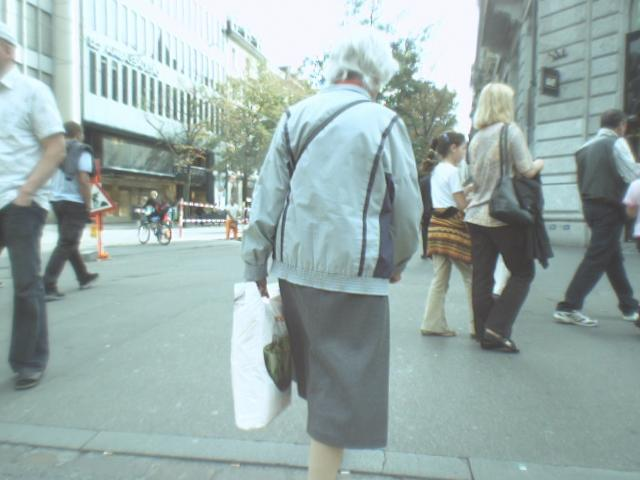
\includegraphics[scale=0.2]{figures/000334.jpg}
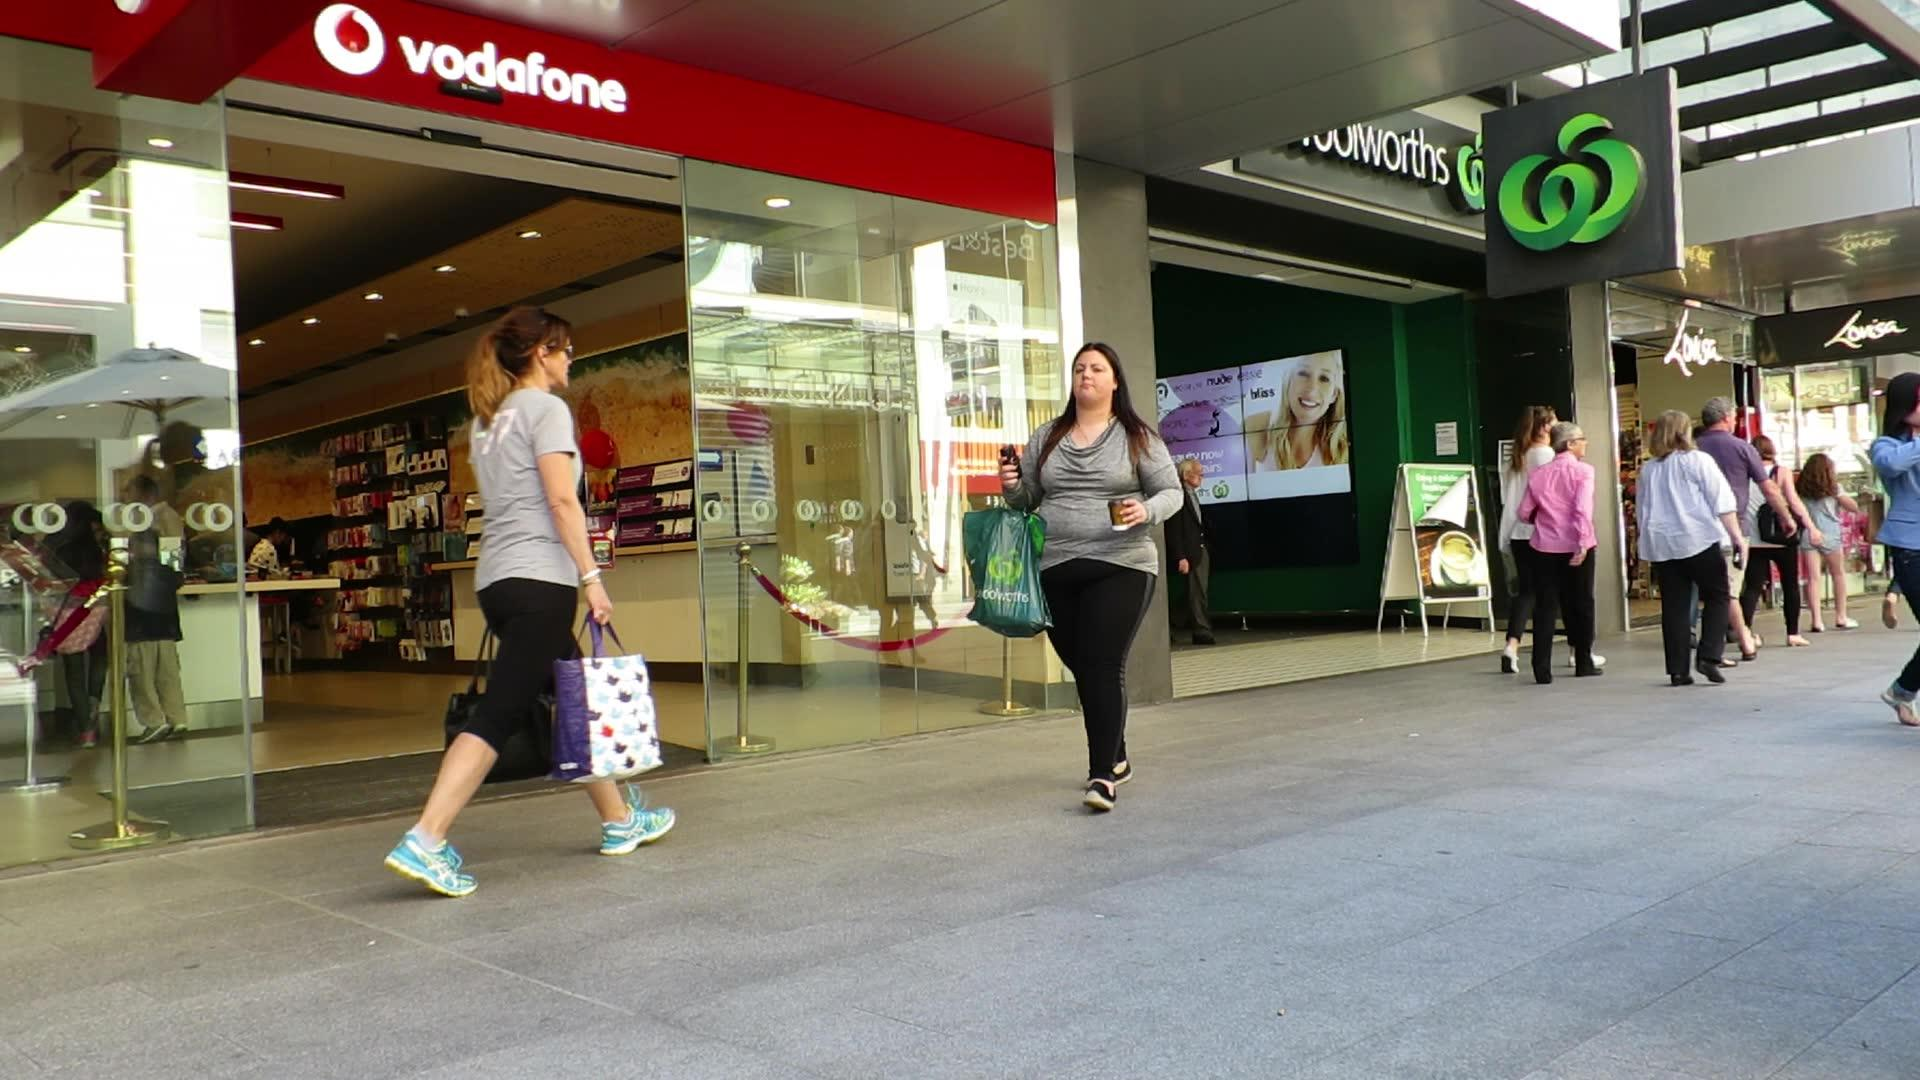
\includegraphics[scale=0.08]{figures/000388.jpg}
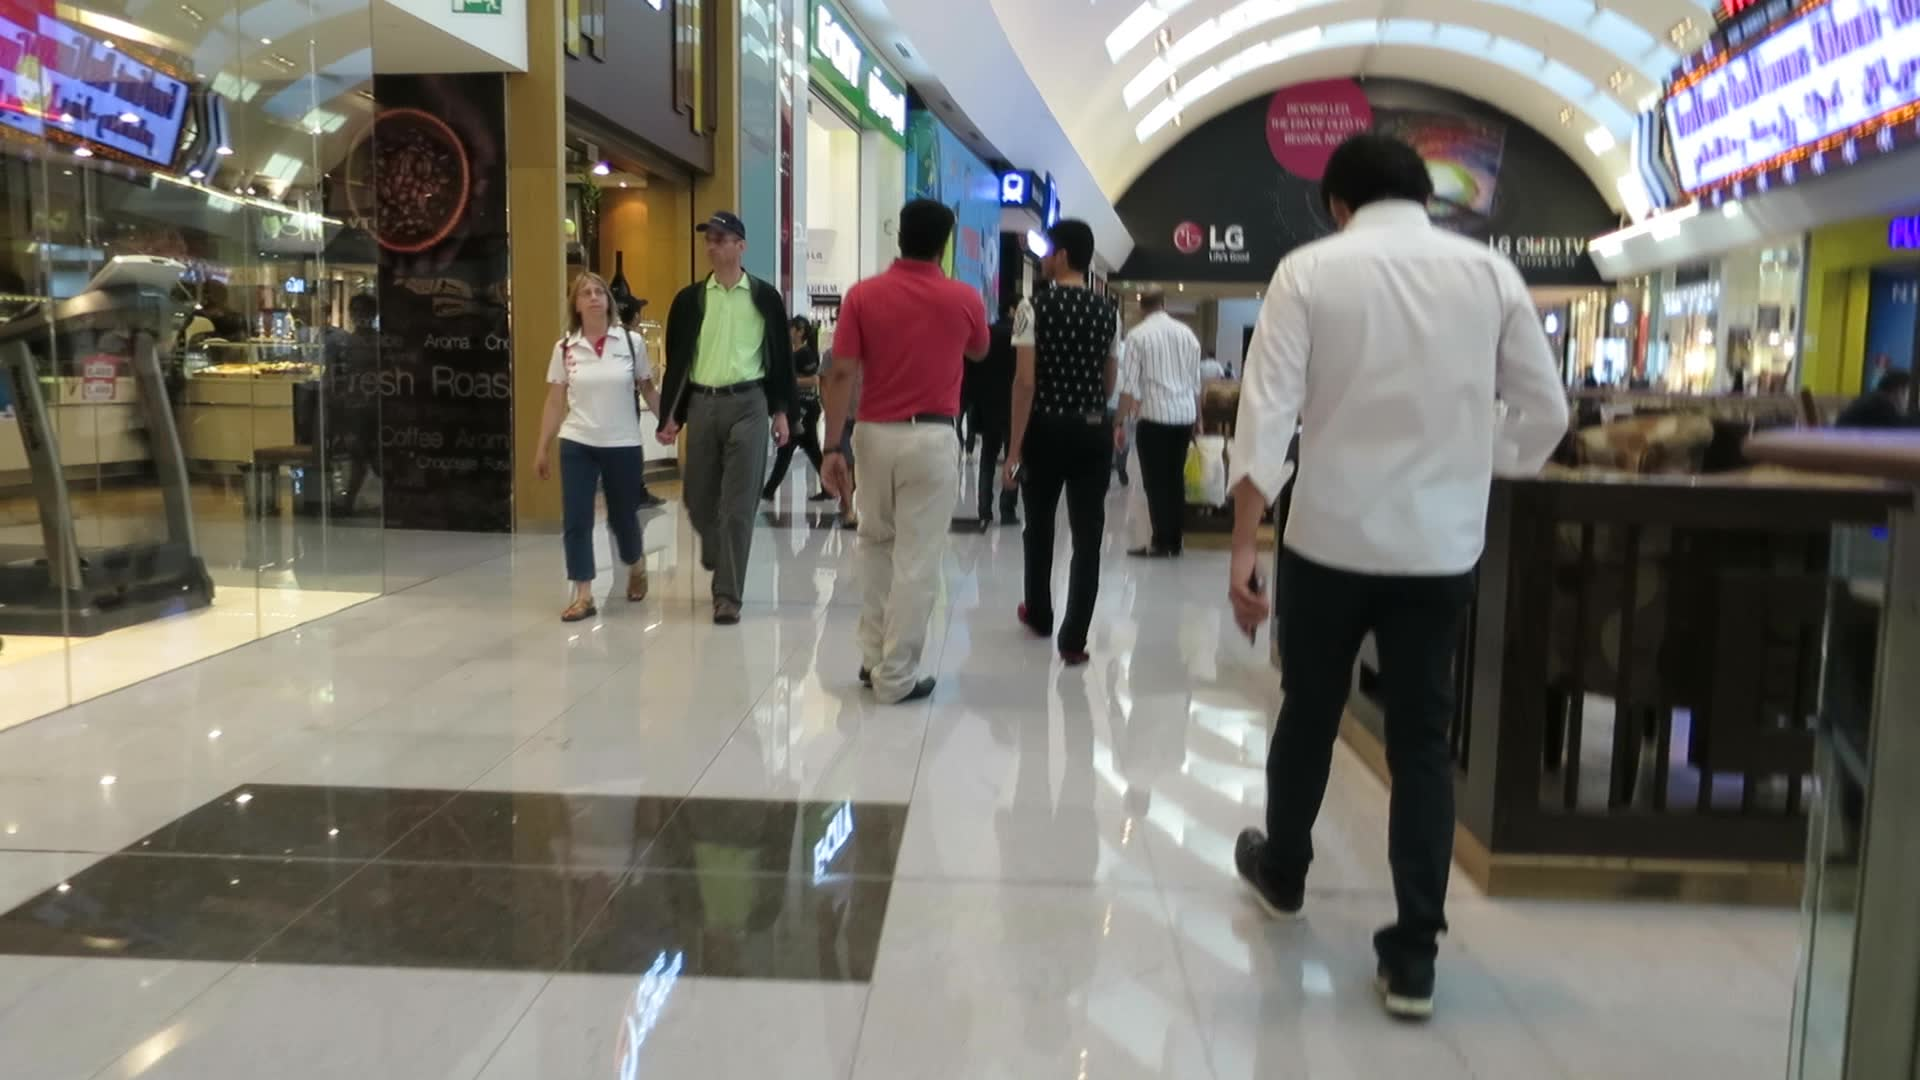
\includegraphics[scale=0.08]{figures/000487.jpg}
\caption{MOT17Det train set samples: left image from MOT17-05, center image from MOT17-09 and right image from MOT17-11}
\label{fig:mot_images}
\end{center}
\end{figure}
The MOSSE tracker was selected as regular tracker and the threshold for all neural network detection was fixed to 0,6. This was done to allow a fair comparison between the models.\\
The MOT17-09 sequence has a fixed camera with several pedestrians walking in groups or alone. In this sequence, the tracking may find fast motion difficulties as well as continuous people coming in and out from the scene. To evaluate the performance in that sequence, two input image sizes were selected due to the Keras SSD-VGG fixed image input size.\\ From the table \ref{tab:net_exp_1}, it can be seen that the maximum AP value is obtained by the Faster R-CNN using 512x512 whereas Mask R-CNN gets the best AP score for 300x300 images. As expected, the R-CNN detectors obtain the best accuracy. However, this accuracy is not linked with the speed in the object detection. The SSD MobileNetV2 gets the best speed rate in both experiments.\\
\begin{table}[H]
\scriptsize
\begin{center}
\begin{tabular}{|c|c|c|}
\hline
\textbf{}                         & \textbf{AP @ 0,5 (\%)} & \textbf{FPS Net} \\ \hline
\textbf{SSD MobileNetV2}          & 16,06                  & 5,282            \\ \hline
\textbf{Faster R-CNN InceptionV2} & 31,03                  & 1,026            \\ \hline
\textbf{Mask R-CNN InceptionV2}   & 27,89                  & 0,286            \\ \hline
\textbf{SSD VGG 512}              & 23,76                  & 0,339            \\ \hline
\end{tabular}
\end{center}
\caption{Experiments on MOT17-09 sequence with 512x512 images}
\label{tab:net_exp_1}
\end{table}
\begin{table}[H]
\scriptsize
\begin{center}
\begin{tabular}{|c|c|c|}
\hline
\textbf{}                         & \textbf{AP @ 0,5 (\%)} & \textbf{FPS Net} \\ \hline
\textbf{SSD MobileNetV2}          & 11,48                  & 8,25             \\ \hline
\textbf{Faster R-CNN InceptionV2} & 24,36                  & 1,067            \\ \hline
\textbf{Mask R-CNN InceptionV2}   & 26,25                  & 0,292            \\ \hline
\textbf{SSD VGG 300}              & 19,08                  & 0,988            \\ \hline
\end{tabular}
\end{center}
\caption{Experiments on MOT17-09 sequence with 300x300 images}
\label{tab:net_exp_2}
\end{table}
The influence of the image input size in the processing speed and the accuracy of the models is clear. The smaller the input size of the image the faster the detections are obtained. In the opposite way, with a bigger input image the final AP result is better. This trend will be confirmed in following experiments.\\

The SSD-VGG models were discarded from other experiments due to its lack of flexibility about the input image size. In the table \ref{tab:net_exp_3}  it can be observed the different performances for 800x800 images of the region-based object detectors and the single-shot object detectors. As it ocurred with smaller image input sizes, the region-based models have a better AP performance almost doubling the AP obtained by the SSD (in the case of Mask R-CNN). For this reason, the SSD MobileNet V2 was eliminated from the neural net selection procedure despite being the fastest. 
\begin{table}[H]
\scriptsize
\begin{center}
\begin{tabular}{|c|c|c|}
\hline
\textbf{}                         & \textbf{AP @ 0,5 (\%)} & \textbf{FPS Net} \\ \hline
\textbf{SSD MobileNetV2}          & 17,13                  & 7,372             \\ \hline
\textbf{Faster R-CNN InceptionV2} & 32,00                  & 0,981            \\ \hline
\textbf{Mask R-CNN InceptionV2}   & 34,23                  & 0,272            \\ \hline
\end{tabular}
\end{center}
\caption{Experiments with 800x800 images}
\label{tab:net_exp_3}
\end{table}
The final experiments were done with Faster R-CNN and Mask R-CNN in MOT17-09, MOT17-11 and MOT17-05. The last two sequences have a common characteristic which is that the camera is in motion. Thus, the sequences are enumerated in order of increasing degree of motion, starting from MOT-09 to MOT-05.
\begin{table}[H]
\scriptsize
\begin{center}
\begin{tabular}{|c|c|c|c|}
\hline
\textbf{AP @ 0,5 (\%)}            & \textbf{MOT17-09} & \textbf{MOT17-11} & \multicolumn{1}{l|}{\textbf{MOT17-05}} \\ \hline
\textbf{Faster R-CNN InceptionV2} & 35,25             & 26,21             & 19,51                                  \\ \hline
\textbf{Mask R-CNN InceptionV2}   & 31,74             & 26,44             & 12,98                                  \\ \hline
\end{tabular}
\end{center}
\caption{Neural network experiments with an image input size of 1000x1000}
\label{tab:net_exp_4}
\end{table}
From these experiments on table \ref{tab:net_exp_4}, it can be seen that the final average precision is similar in the sequence MOT17-11, however, the use of Faster R-CNN model outperforms Mask R-CNN in the other two sequences. These AP scores can be related with the frame rate obtained from each neural network which is about 0,9 FPS for Faster R-CNN and 0,2 FPS for Mask R-CNN. A higher speed can help the tracking procedure to be ``refreshed" more frequently which may lead to better performance on sequences with varying motion between frames as it occurs on the evaluated sequences.\\ In the figure \ref{fig:faster_dets} it can be observed an example of the detections obtained with Faster R-CNN. Generally, the results seem to be pretty accurate but they include some false positives such as the person assigned to a confidence of the 69\%.\\
Given these cuantitative results, the final neural network chosen to perform the object detection in dl-objecttracker is Faster R-CNN InceptionV2.
\begin{figure}[H]
\begin{center}
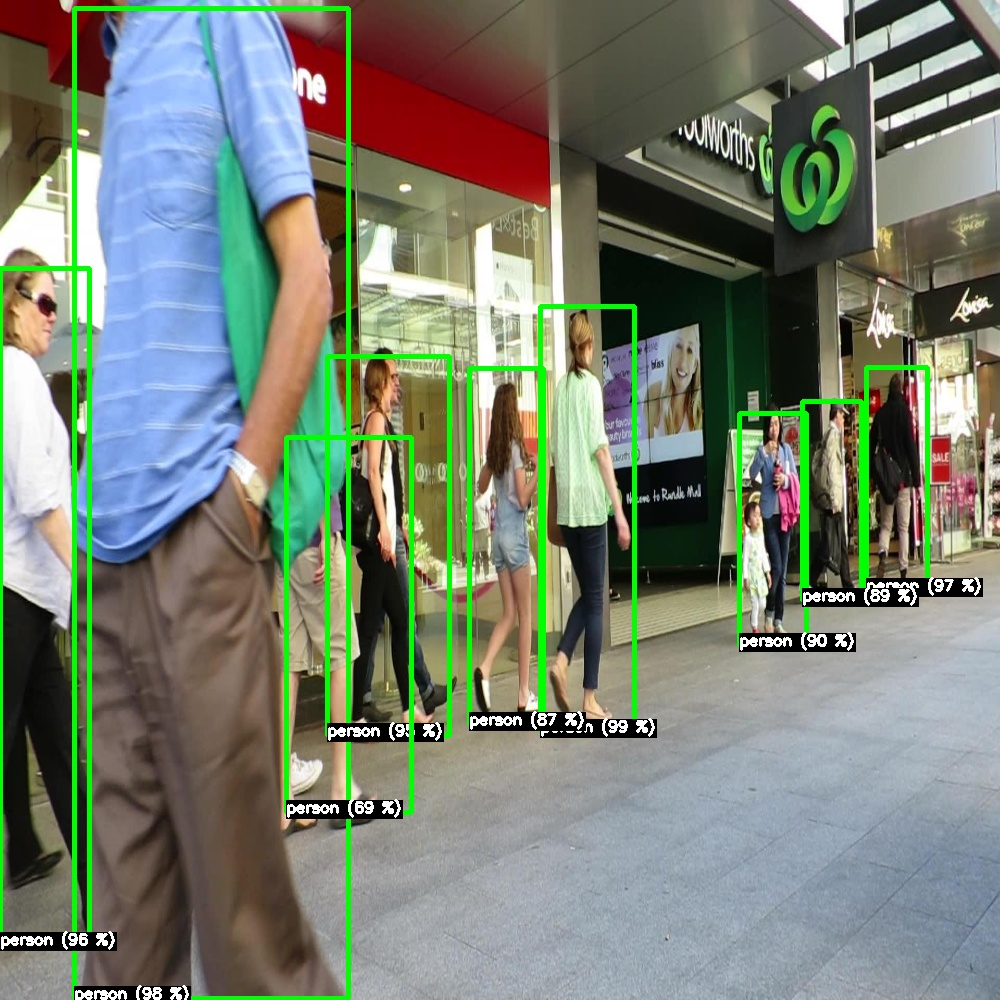
\includegraphics[scale=0.2]{figures/212.jpg}
\caption{Faster R-CNN Inception V2 object detections on MOT17-09}
\label{fig:faster_dets}
\end{center}
\end{figure}
\section{Tracker's performance}
Once the neural network was selected, it is time to evaluate the performance of the second module involved in the core of the multiobject tracking application, the tracking module.\\
The following experiments were done on the same sequences as the Network experiments. In this case, the default configuration includes Faster R-CNN as neural network with a confidence threshold for detection set to 0,6. The confidence of the tracker is being used if no comment is made on it. This confidence is going to be modified later in this section to see its influence on the results. The following tracking algorithms were evaluated: KCF, BOOSTING, MIL, TLD, MEDIANFLOW, CSRT, MOSSE and CF-dlib (section \ref{tracker_algorithms}).\\
\begin{table}[H]
\scriptsize
\begin{center}
\begin{tabular}{|c|c|c|}
\hline
\textbf{}           & \textbf{AP @ 0,5 (\%)} & \textbf{FPS Tracker} \\ \hline
\textbf{KCF}        & \textit{23,07}         & \textit{6,39}        \\ \hline
\textbf{BOOSTING}   & 13,06                  & 4,78                 \\ \hline
\textbf{MIL}        & 15,29                  & 2,21                 \\ \hline
\textbf{TLD}        & 8,38                   & 2,22                 \\ \hline
\textbf{MEDIANFLOW} & \textit{32,13}         & \textit{12,01}       \\ \hline
\textbf{CSRT}       & 11,78                  & 2,78                 \\ \hline
\textbf{MOSSE}      & \textit{34,60}         & \textit{47,07}       \\ \hline
\textbf{CF-dlib}    & \textit{27,99}         & \textit{9,51}        \\ \hline
\end{tabular}
\end{center}
\caption{Tracker experiments on MOT17-09 sequence with 1000x1000 images}
\label{tab:tracker_exp_1}
\end{table}
This experiment provides clear results on the performance of the trackers in the MOT17-09 sequence. The KCF, MEDIANFLOW, MOSSE and CF-dlib outperform in a significant way the accuracy of the rest of the trackers (in terms of AP). A good AP seems to be related with a good frame rate in the tracking.\\
The scheme of evaluating the performance with sequences of increasing difficulty was followed, the second experiment was performed with the MOT17-11 sequence and its results are shown in table \ref{tab:tracker_exp_2}.

\begin{table}[H]
\scriptsize
\begin{center}
\begin{tabular}{|c|c|c|}
\hline
\textbf{}           & \textbf{AP @ 0,5 (\%)} & \textbf{FPS Tracker} \\ \hline
\textbf{KCF}        & 19,17                  & 4,7                  \\ \hline
\textbf{MEDIANFLOW} & \textit{27,76}         & \textit{12,88}       \\ \hline
\textbf{MOSSE}      & \textit{26,23}         & \textit{33,56}       \\ \hline
\textbf{CF-dlib}    & \textit{25,49}         & \textit{9,95}        \\ \hline
\end{tabular}
\end{center}
\caption{Tracker experiments on MOT17-11 sequence with 1000x1000 images}
\label{tab:tracker_exp_2}
\end{table}
The results in this sequence seem to indicate that the KCF tracker is not adecuated for the task. Its results in both AP and the speed measurements are below the overall average.
\begin{table}[H]
\scriptsize
\begin{center}
\begin{tabular}{|c|c|c|}
\hline
\textbf{}           & \textbf{AP @ 0,5 (\%)} & \textbf{FPS Tracker} \\ \hline
\textbf{MEDIANFLOW} & \textit{24,01}         & \textit{13,05}       \\ \hline
\textbf{MOSSE}      & 16,15                  & 18,14               \\ \hline
\textbf{CF-dlib}    & 23,97                  & 9,51                 \\ \hline
\end{tabular}
\end{center}
\caption{Tracker experiments on MOT17-05 sequence with 1000x1000 images}
\label{tab:tracker_exp_3}
\end{table}
The results from table \ref{tab:tracker_exp_2} led us to three final tracker options: MEDIANFLOW, MOSSE and CF-dlib. In the experiment on MOT17-05 shown on table \ref{tab:tracker_exp_3}, MEDIANFLOW gets the overall best performance. It achieves the highest AP score of the three tracker options and the second faster tracking. The faster tracker is MOSSE, following the trend of previous experiments.
\subsection{Confidence in tracking}
In section \ref{conf_in_tracking}, the mechanism of confidence of the tracker was introduced. The tracker itself continuously checks if the tracking obtained for each object is reliable enough. In this section, the importance of this parameter is going to be evaluated. To do so, the performance of the three best tracking algorithms is measured when the confidence is taken into account and in the opposite case. The selected sequences are MOT17-05 and MOT17-09 with a frame size of 500x500 and the neural network used in both cases is Faster R-CNN InceptionV2.\\
\begin{table}[H]
\scriptsize
\begin{center}
\begin{tabular}{|c|c|c|}
\hline
\textbf{}           & \textbf{AP tracker on @ 0,5 (\%)} & \textbf{AP tracker off @ 0,5 (\%)} \\ \hline
\textbf{MEDIANFLOW} & 36,09                             & 32,35                              \\ \hline
\textbf{MOSSE}      & 18,60                             & 10,33                              \\ \hline
\textbf{CF-dlib}    & 23,74                             & 30,06                              \\ \hline
\end{tabular}
\end{center}
\caption{Confidence influence on tracking performance on MOT17-05}
\label{tab:tracker_exp_4}
\end{table}
\begin{table}[H]
\scriptsize
\begin{center}
\begin{tabular}{|c|c|c|}
\hline
\textbf{}           & \textbf{AP tracker on @ 0,5 (\%)} & \textbf{AP tracker off @ 0,5 (\%)} \\ \hline
\textbf{MEDIANFLOW} & 37,80                             & 36,17                              \\ \hline
\textbf{MOSSE}      & 30,16                             & 21,83                              \\ \hline
\textbf{CF-dlib}    & 28,06                             & 31,60                              \\ \hline
\end{tabular}
\end{center}
\caption{Confidence influence on tracking performance on MOT17-09}
\label{tab:tracker_exp_5}
\end{table}
In the tables \ref{tab:tracker_exp_4} and \ref{tab:tracker_exp_5} the results seem to indicate that the influence of taking into account the confidence parameter with OpenCV trackers is positive. However, it occurs the opposite for the \texttt{dlib} tracking with CF.\\
The MEDIANFLOW tracker was finally selected to perform the tracking in the dl-objecttracker application given the performace shown in the previous experiments. Figure \ref{fig:medianflow_images} shows an example of the tracking using that tracking algorithm.\\
Finally, the image input size was modified to check which size was best appropriate to our problem. In table \ref{tab:annex_1} of the \textit{Annex}, the image size of 400x400 gets the best balance between speed and accuracy for the tracking task. Given the tracker and the image size, the threshold for the confidence of the detections from the object detection neural networks was evaluated. Using values ranging from 0,3 to 0,7 the experimental threshold selected was 0,5.
\begin{figure}[H]
\begin{center}
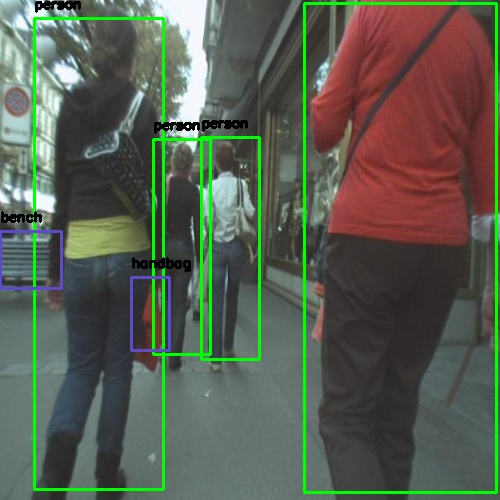
\includegraphics[scale=0.25]{figures/652.jpg}
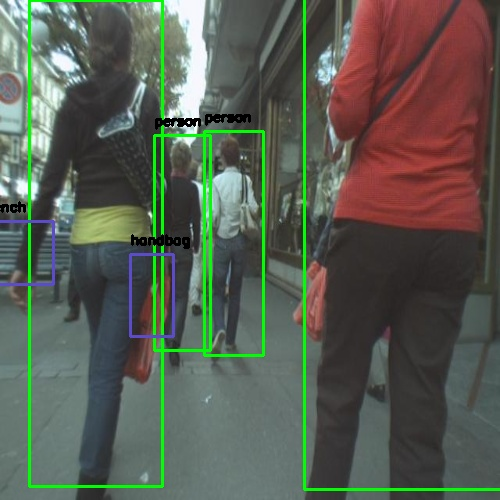
\includegraphics[scale=0.25]{figures/655.jpg}
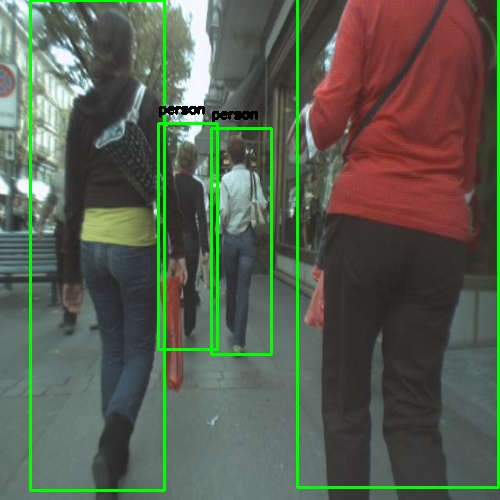
\includegraphics[scale=0.25]{figures/659.jpg}
\caption{Medianflow multiobject tracking on MOT17-05 (selected frames are not sequential)}
\label{fig:medianflow_images}
\end{center}
\end{figure}
\subsection{GOTURN tracking}
The GOTURN (\textit{Generic Object Tracking Using Regression Networks}) is a deep learning based tracking algorithm which learns the motion of the object in an \textit{offline} manner. Many real-time trackers rely on \textit{online} learning that is usually much faster than a deep learning based tracking solution. The authors claim in the original paper \cite{held2016learning} that their system is ``the first neural-network tracker that learns to track generic objects at 100 FPS" (using GPU acceleration, Nvidia GTX 680). However, when using only a CPU the tracker runs at 2,7 FPS according to the authors. This was the main reason to discard this tracker for the project. 
\section{Experimental validation of the final solution}\label{final_sol}
After the unit test experiments, the dl-objecttracker application follows this configuration:
\begin{enumerate}
    \item Neural network: Faster R-CNN InceptionV2, image input size 400x400, confidence threshold 0,5
    \item Tracker: MedianFlow using tracking confidence
\end{enumerate}
Given this configuration, the whole application was evaluated on the complete train set of MOT17Det to obtain the results of our final solution.
\begin{table}[H]
\begin{center}
\begin{tabular}{|c|c|c|c|}
\hline
\textbf{dl\_objecttracker} & \textbf{AP @ 0,5 (\%)} & \textbf{FPS Net} & \multicolumn{1}{l|}{\textbf{FPS Tracker}} \\ \hline
\textbf{MOT17-02}          & 11,59                  & 0,93             & 31,4                                      \\ \hline
\textbf{MOT17-04}          & 17,25                  & 0,869            & 23,96                                     \\ \hline
\textbf{MOT17-05}          & 36,53                  & 0,98             & 37,28                                     \\ \hline
\textbf{MOT17-09}          & 43,53                  & 0,95             & 35,83                                     \\ \hline
\textbf{MOT17-10}          & 23,26                  & 0,943            & 36,18                                     \\ \hline
\textbf{MOT17-11}          & 35,74                  & 0,96             & 41,56                                     \\ \hline
\textbf{MOT17-13}          & 14,04                  & 0,941            & 42,01                                     \\ \hline
\end{tabular}
\end{center}
\caption{Final results on MOT17Det train set}
\label{tab:final}
\end{table}
The best results in terms of average precision occur in the MOT17-09 sequence, followed by MOT17-11 and MOT17-05. This may indicate that the procedure used influences the results giving the better scores in the sequences used to evaluate the performance of the Tracker and Network module. However, from table \ref{tab:annex_2} and table \ref{tab:annex_3} it can be observed that the three mentioned sequences have in common that they have a small number of total ground truth ocurrences. It can be easier for the developed system to get good results in this type of sequences. The results indicate that the developed application performs best on sequences with lowly crowded densities.\\
Refering to the speed of the developed application, the object detection in the neural network is returned with a stable frame rate of about 1 FPS and the tracker runs above 20 FPS in every sequence.

\lhead[]{CHAPTER \thechapter. Conclusions}
\chapter{Conclusions}
This chapter summarizes the main contributions of this work. Finally, possible lines of future work are outlined.\\
This master thesis studied the use of deep learning techniques to build a multiobject tracking system using the tracking-by-detection scheme. To solve this task we used a modular architecture composed of a Network module, a Tracker module, a Camera module and a GUI module. The first module provides object detections using neural network models. These detections are handled by the Tracker module to track a buffer of frames before the new detections had come from the Network. The Camera module controls the general flow of the project which includes the logging mechanism and the user interface (GUI), among others.\\
The Tracker module can work on three operating regimes depending on the frame rate of the tracking at each instance of time: slow, normal and fast. This allows the tracking to adapt its speed to the processing difficulties (different image sizes, occlusions, appearance changes, ...). It may also help to adapt the speed to the hardware on which it is being used.
Refering to the user side, the project application allows the user to change many configuration options. This feature can help the quick test of neural networks or trackers for multiobject tracking tasks, for example.\\
Once the multiobject tracking system was developed, the first three objectives (section \ref{first_objective}) were fullfilled:
\begin{enumerate}
    \item Development of an object detector using deep learning
    \item Development of a tracking module
    \item Combination of neural object detection and object tracking in a single component
\end{enumerate}
After this, the last objective was accomplished as the component was evaluated on a well-known multiobject tracking dataset (MOT17Det) allowing us to choose the best configuration based on some experiments. This included the selection of a neural network model, a tracking algorithm and other parameters such as the confidence thresholds or the image input size (section \ref{final_sol}). The performance and speed measurements obtained allowed us to extract the following conclusions:
\begin{itemize}
    \item Region-based object detection neural networks obtain better accuracy than single-shot based ones. They can be used to perform inference on CPU at low frame rates.
    \item MedianFlow seems to be the best tracker available in the OpenCV library for its balance between speed and accuracy. MOSSE is the fastest one.
    \item The confidence is useful to discard bad tracking performance when working with OpenCV trackers. However, dlib tracking seems to be less influenced by the confidence thresholding.
    \item The image input size is a key factor when working with resource limited hardware to achieve higher throughput.
    \item The final solution seems to perform better on sequences with lower crowd density.
\end{itemize}
We can say that we have built a multiobject tracking system that performs reasonably well on a MOT dataset despite not being into the State-of-the-Art.
\section{Future work}
This master thesis is a first step into the multi-object tracking with deep learning. Once developed and seen the results, we propose the following lines of future work:
\begin{enumerate}
    \item Train neural network models used (or new ones) in multiobject tracking datasets such as MOT. This could lead to better results.
    \item Refering to the tracking, the multiprocessing with dlib for tracking is available but it was not introduced in the project. This may speed up the tracking with dlib.
    \item Obtain the best configuration in a different way. For example, trying more possible combinations of parameters in other dataset sequences.
    \item Improve the metrics calculation by assigning IDs to the tracked objects allowing for the calculation of tracking metrics (MOTA, for example). There exists official Python implementations of metrics for benchmarking MOT such as \href{https://github.com/cheind/py-motmetrics}{\textit{py-motmetrics}}.
    \item Test the application in other non-GPU devices as Raspberry Pi or Intel Computer Stick and in devices with graphic acceleration.
    \item Try weights quantization techniques in neural networks with high number of parameters (region-based, for example). It can help to speed up the inference time and it will be more efficient in terms of memory consumption.
\end{enumerate}

\lhead[]{BIBLIOGRAPHY}
\phantomsection
\addcontentsline{toc}{chapter}{Bibliography}
\bibliographystyle{unsrt}
\bibliography{egbib}

\end{document}
